
%%%%%%%%%%%%%%%%%%%%%%%%%%%%%%%%%%%%%%%%%%%%%%%%%%%%%%%
%%% code: 代码文件夹
%%% figures: 图片文件夹
%%% *.cls: LaTeX 格式文件
%%% *.tex: LaTeX 文档文件
%%% *.bib: Bib 引用文献源文件
%%%%%%%%%%%%%%%%%%%%%%%%%%%%%%%%%%%%%%%%%%%%%%%%%%%%%%%

%%%%%%%%%%%%%%%%%%%%%%%%%%%%%%%%%%%%%%%%%%%%%%%%%%%%%%%
%%% 可能用到的网站
%%%%%%%%%%%%%%%%%%%%%%%%%%%%%%%%%%%%%%%%%%%%%%%%%%%%%%%
%%% LaTeX公式编辑器:https://www.latexlive.com/
%%% Diagram流程图绘制:https://www.drawio.com/
%%%%%%%%%%%%%%%%%%%%%%%%%%%%%%%%%%%%%%%%%%%%%%%%%%%%%%%
\documentclass{mcmthesis}  % 文档类型
\mcmsetup{CTeX = false,   % 使用 CTeX 套装时,设置为 true
        tcn = 2407527,   % 队伍控制号
        problem = c,  % 选题
        sheet = true,   % sheet页
        titleinsheet = true,   % sheet页显示标题
        keywordsinsheet = true,  % sheet页显示关键词
        titlepage = false,   % 标题页
        abstract = true  % 摘要
        }
\makeatletter
\newcommand{\rmnum}[1]{\romannumeral #1}
\newcommand{\Rmnum}[1]{\expandafter\@slowromancap\romannumeral #1@}
\makeatother
%%%%%%%%%%%%%%%%%%%%%%%%%%%%%%%%%%%%%%%%%%%%%%%%%%%%%%%

%%%%%%%%%%%%%%%%%%%%%%%%%%%%%%%%%%%%%%%%%%%%%%%%%%%%%%%
%%% 导入宏包和引用文献源
%%%%%%%%%%%%%%%%%%%%%%%%%%%%%%%%%%%%%%%%%%%%%%%%%%%%%%%
\usepackage{palatino}  % 帕拉提诺体字体宏包
\usepackage{lipsum}  % 导入生成段落的宏包
\usepackage[hyperref=true,style=ieee]{biblatex}  % biblatex参考文献宏包
\usepackage{float}
\addbibresource{ref.bib}  % 添加引用文献bib源
\usepackage{amssymb} %罗马数字包
\usepackage{stfloats}
%%%%%%%%%%%%%%%%%%%%%%%%%%%%%%%%%%%%%%%%%%%%%%%%%%%%%%%

%%%%%%%%%%%%%%%%%%%%%%%%%%%%%%%%%%%%%%%%%%%%%%%%%%%%%%%
%%% 文档信息设置
%%%%%%%%%%%%%%%%%%%%%%%%%%%%%%%%%%%%%%%%%%%%%%%%%%%%%%%
\title{The Magical Force Determining Fate in Tennis------"Momentum"}  % 文章标题
\author{\small Team 2407527}  % 作者,开启标题页才会显示
\date{\today}  % 日期,开启标题页才会显示

%%%%%%%%%%%%%%%%%%%%%%%%%%%%%%%%%%%%%%%%%%%%%%%%%%%%%%%

%%%%%%%%%%%%%%%%%%%%%%%%%%%%%%%%%%%%%%%%%%%%%%%%%%%%%%%
%%% 文档开始
%%%%%%%%%%%%%%%%%%%%%%%%%%%%%%%%%%%%%%%%%%%%%%%%%%%%%%%
\begin{document}  % 文档
\thispagestyle{empty}
\begin{abstract}  % 摘要
\par In tennis, momentum is described as the strength or confidence gained through events, which is the psychological and physiological state of players. The transformation of momentum is a key factor in determining the victory. We first establish a mathematical model of momentum and study the correlation between momentum and outcome. Based on this, we establish a model to measure player performance and predict the transition point of the competition situation. Study of this issue can provide tactical and training guidance for players and coaches to predict the game situation and to performance well .

\par The \textbf{first} model is to measure the performance of tennis players in a match. It is influenced by three factors: athlete's technical ability, fatigue level, and momentum. We first constructed a momentum model and considered the influence of multiple factors on momentum, including scoring factors, serving factors,  etc. By setting weight, we quantified the \textbf{concept of momentum}. Subsequently, we used \textbf{logistic regression} to establish a model for measuring the performance of athletes, with an accuracy of \textbf{0.694} was visualized and presented. We conducted a significance test on the eleven performance factors of logistic regression using \textbf{SPSS}, and found that five indicators had a significant impact on the scores of athletes, such as leading score, order of hand, running distance, etc. At the same time, the \textbf{Bayes model} was used for comparison and it was found that the logistic regression model is more suitable. Finally, we used \textbf{Pearson} correlation test and successfully demonstrated a significant correlation between momentum and score.

\par The second model is to predict turning points in tennis matches. We define the moment when momentum changes sharply as the turning point and use \textbf{random forest model} for prediction, achieving an accuracy of \textbf{0.686}. We visualized the prediction results and studied the importance of each indicator, and found that running distance, order, and score leadership have the \textbf{greatest impact} on the turning point . Therefore, we have put forward some suggestions, including strategies such as Inducing opponents to run more, reducing one's own running distance, and providing differentiated suggestions for specific athletes.

\par Finally, we conducted model extension testing to verify its \textbf{generalization ability}. By using our model on previous male/female singles datasets for prediction, the results show that the model performs well .However, When applied to other fields, some indicators, such as breaking rate, may not exist and the rules may be different. We provide some suggestions, including transforming features, adding more rules, etc.

\begin{keywords}  % 关键词
Tennis, Logistic regression, Random forest, Tennis
\end{keywords}  % 结束关键词
\end{abstract}  % 结束摘要


\maketitle  % 生成sheet页

\tableofcontents  % 生成目录表

%%%%%%%%%%%%%%%%%% sheet页与目录页结束 %%%%%%%%%%%%%%%%%%

\newpage  % 开始新的一页
\section{Introduction}  % 一级标题
\subsection{Problem Background}  % 二级标题
\hspace{1.5em}In the 2023 Wimbledon Gentlemen's final, the young and talented 20-year-old Spanish player, Carlos Alcaraz, achieved a stunning victory over the seasoned 36-year-old Novak Djokovic. The match itself was nothing short of extraordinary with its roller coster-like score between the two players.
\par The remarkable shifts, occasionally spanning numerous points or even entire games, observed in the player who appeared to be in control are frequently ascribed to the concept of "momentum."In sports, momentum is described as the "strength or force gained by motion or a series of events."
\par The acquisition of momentum is vital in tennis as it provides the player with a feeling of command and places pressure on the opponent to regain control. When a player gains momentum, they tend to play with increased freedom, exhibiting less fear and inhibition. This often translates into a more aggressive and confident playing style. \cite{jesse2016}
\par Capturing and measuring this force during a match or game can be challenging. Additionally, understanding how various events contribute to the creation or alteration of momentum remains a complex and intriguing aspect of sports analysis.
\par Now, let's explore how we can analyze momentum in tennis and how to utilize it well!


\subsection{Our work}  % 二级标题  
\hspace{1.5em}1. For 1, 2 questions, we want to build a regression model to capture the changing situation of the scene and measure the real-time performance of the players. We studied many factors to quantify the concept of "momentum" .Next,we used a logistic regression model .We considered momentum  and other factors as independent variables and whether they could be scored as dependent variables. Finally, use the matplotlib library to visualize the player's performance.%段落前空格
\par2. Then, through Pearson correlation test and visualization processing of momentum and outcome in the model, we proved the correlation between momentum and results of the matches to the tennis coach, thus proving that momentum and outcome played a key role in the match.
\par3. We believe that the turning point in the game is the huge momentum transition point of the player. Based on the momentum model, the turning point is determined by  according to the speed of momentum changing. Then the characteristic results are analyzed by Random Forest, and the game styles of different players are analyzed, and the general suggestions and suggestions for players are put forward.
\par4. We test the model on other data sets to verify the model's generalization of data. The model extends from special to general, from men's tennis field to women's tennis, table tennis, badminton and so on. The ideas and methods of model expansion for other types of sports competitions are also given.
\par5. Finally, we summarize a memo report, propose the role of momentum in tennis matches, and give some strategy suggestions for tennis players

\section{Assumptions}  % 一级标题
\hspace{1.5em}To simplify our model and reduce complexity, we make the following assumptions in the paper.
\par 
1. Server advantage hypothesis: The server is more likely to win points than the receiver, which will affect the outcome.\cite{ZGTK202311031139}\par 
2. Momentum influence hypothesis: A player's performance is affected by momentum in the race, and past success or failure will affect future performance.\par  
3. Stable condition assumption: the type and condition of the tennis court are fixed and will not change with the weather, temperature, humidity and other factors.\cite{SPOR202304012}\par  
4. The assumption of fairness of the match environment: the referee of the tennis match is fair, and the sponsors and media of the match will not interfere with the players due to commercial interests or public opinion.


%%%%%%%%%%%%%%%%%%%%%%%% 并排图 %%%%%%%%%%%%%%%%%%%%%%%%
%\begin{figure}[h]  % 图片
%\centering  % 居中
%\begin{minipage}[c]{0.48\textwidth}  % 子页
%\centering  % 居中
%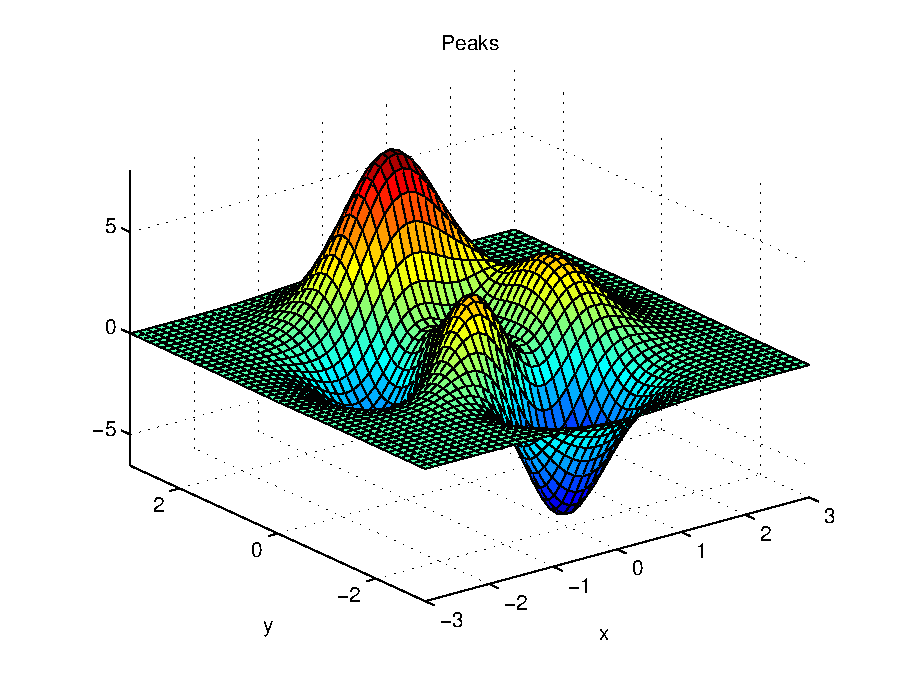
\includegraphics[width=7cm]{example.eps}  % 引入图片源
%\caption{example2} \label{fig:example}  % 标题与标签
%\end{minipage}  % 子页结束
%\hspace{0.02\textwidth}
%\begin{minipage}[c]{0.48\textwidth}  % 子页
%\centering  % 居中
%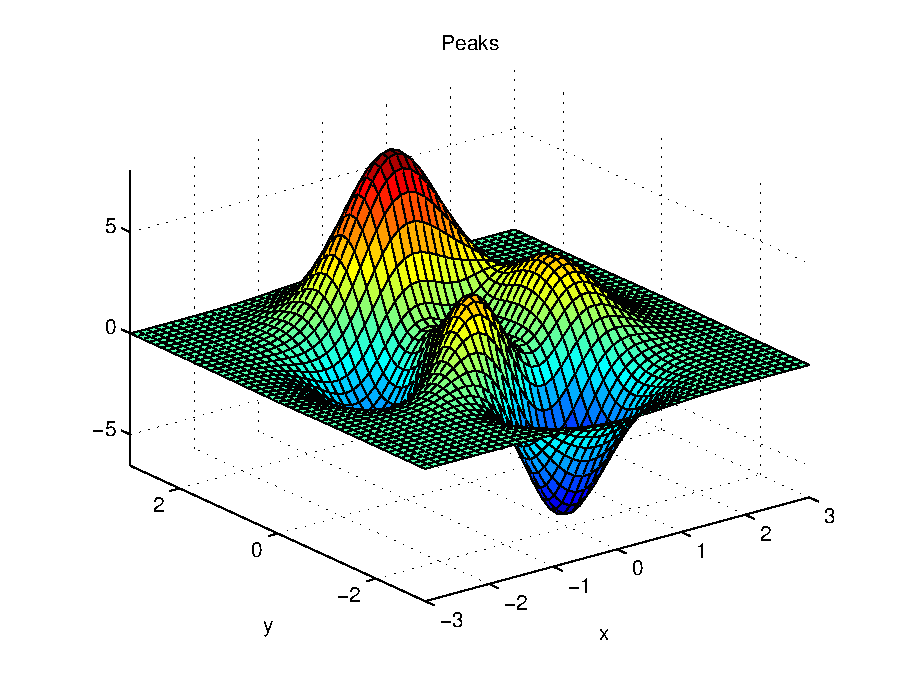
\includegraphics[width=7cm]{example.eps}  % 引入图片源
%\caption{example3} \label{fig:example}  % 标题与标签
%\end{minipage}  % 子页结束
%\end{figure}  % 图片结束
%%%%%%%%%%%%%%%%%%%%%% 并排图结束 %%%%%%%%%%%%%%%%%%%%%%

%\begin{figure}[h]  % 图片
%\small
%\centering  % 居中
%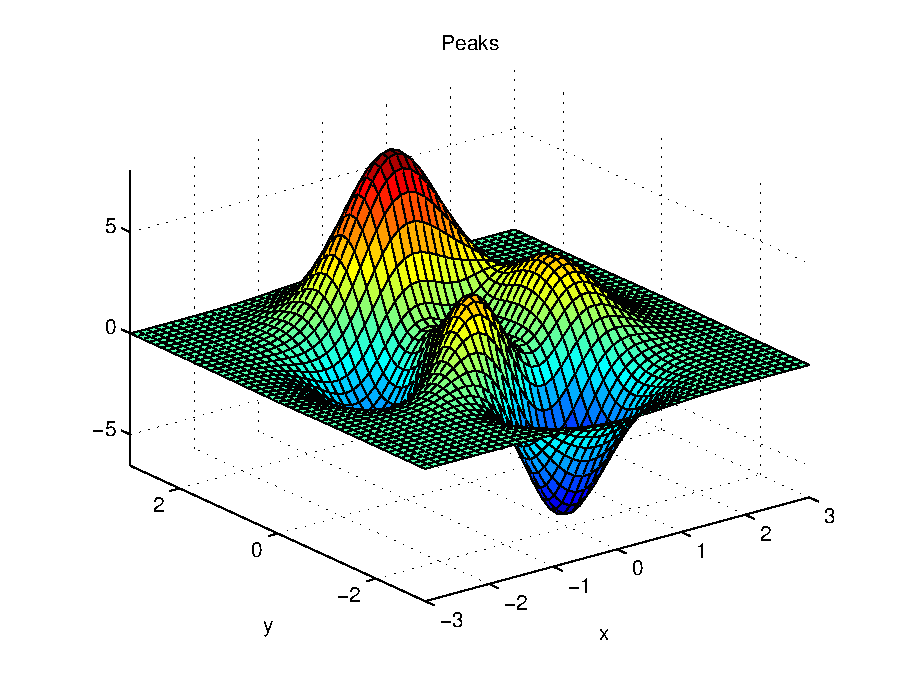
\includegraphics[width=12cm]{example.eps}  % 引入图片源
%\caption{example} \label{fig:example}  % 标题与标签
%\end{figure}  % 图片结束

%This is Figure \eqref{fig:example}.  % 引用图表
%This is table 1 \eqref{tab1}
%This is table 2 \ref{tab2}

%%%%%%%%%%%%%%%%%%%%%% 并排图结束 %%%%%%%%%%%%%%%%%%%%%%
\section{Notations}  % 一级标题

\begin{table}[!htb]  % 表格
\centering
\caption{significance test}  % 标题
\label{tab2}  % 标签
\tabcolsep 50pt % 列间距
\begin{tabular*}{\textwidth}{cl}  % tabular*环境
\toprule  % 顶线
    symbol & illustrate \\
    \midrule  % 中线
        P_{t} & Point winner \\
        S_{t} & Server \\
        n & total number of rounds of the match \\
        I(cdot) & Indicates \\
        \text{diff} & Game difference between players \\
        score_{\text{diff}} & Score difference between players \\
        rally\_{factor} & Normalized number of rounds \\
        distance\_{factor} & normalized running distance \\
        break\_point\_{value} & The basic momentum score increase value \\
        S_{pw} & consecutive scoring \\
        S_{gw} & the number of consecutive winning games \\
        BS_{\text{diff}} & a large score difference \\
        SS_{\text{diff}} & a small score difference \\
        BP & The impact of a break  \\
        R_{factor} & the number of beats  \\
        I({rally\_count} > 10) & multi-goal scoring \\
        I({ACE}) & ACE score \\
        I({unforced\_error}) & The impact of unforced errors \\
    \bottomrule  % 底线
    \end{tabular}
\end{table}

% I(cdot) & Indicates a function that takes the value 1 when the condition in the brackets is true, otherwise it is 0 \\
% break\_point\_{value} & The basic momentum score increase value of break point is initially 1. Each time a break point is missed, it will be reduced by 0.1, with a minimum of 0.1. \\
% R_{factor} & The impact of the number of beats and running distance is \$2.0 times text\{rally\_factor} times text\{distance\_factor} times P\_t \\
% S_{pw} & The impact of consecutive scoring is \$0.03 times text\{consecutive\_point\_wins} \\
% S\_{gw} & The impact of the number of consecutive winning games is \$0.2 times text\{consecutive\_game\_wins} \\
% BS_{diff} & The impact of a large score difference is \$0.1 times 2\^\{diff} \\
% SS_{diff} & The impact of a small score difference is \$0.02 times text\{score\_diff} times P\_t \\
% BP & The impact of a break is break\_point\_value} times P\_t\$ \\
% I({rally\_count} > 10) & The impact of multi-goal scoring is \$0.5\$ \\
% I({ACE}) & The impact of ACE score is \$0.02\$ \\
% I({unforced\_error}) & The impact of unforced errors is \$0.05\$ \\

%%%%%%%%%%%%%%%%%%%%%% 三线表结束 %%%%%%%%%%%%%%%%%%%%%%
% \usepackage{color}



\section{Model \Rmnum{1}:Model for Evaluating Player Performance}
\subsection{Data Preprocessing}

1.\textbf{Categorical Values:}\\
The dataset contains numerous categorical variables in string format. To facilitate regression modeling, we encoded and assigned the values of the last three columns of tennis match.We unified all categorical variables into numerical values for subsequent processing. For instance, converting "AD" in the score to 50, replacing "ND" and "D" with "5" and "15" in the returning depth, and replacing "CTL" and "CT" with "6" and "3" in the serving depth.\cite{ZGTK202311031139}\\

2.\textbf{Abnormal Value:}\\
Abnormal Value can have a detrimental impact on the model. Following the 3-standard deviation rule, the range of outliers is determined, marked, and addressed using mean imputation.We ensure the accuracy and consistency of data, preventing its impact on subsequent analyses and the model.


\subsection{Model for Evaluating Player Performance Construction}
\hspace{1.5em}We reviewed literature investigating the determining factors in tennis matches, categorizing them into three main types: the overall performance of the player, the overall performance of the opponent, and the decisions made by the umpire. Among these, the overall performance of the opponent and the umpire's decisions are beyond the player's control. In contrast, the player's own overall performance is the only aspect they can genuinely influence and control, making it the core factor in ultimately securing victory. 
\par The current determining factors are primarily classified into three types: fatigue level, individual technical ability, and player's state . We  summarized the state as "momentum" .\cite{QSTY202210018}
\begin{itemize}  % 无序列表
\item For individual technical ability, we can calculate it using past or real-time player scoring situations.
\item For player fatigue level, we can calculate it using the player's running distance.
\item Momentum is a force or power gained through motion or a series of events. We use events that can influence player's state such as serving errors, consecutive wins, and direct serving points, to quantify momentum.
\end{itemize}  % 无序列表结束


\begin{table}[ht]
\centering
\caption{Variable}
\begin{tabular}{cl} 
\hline
Variable Name & \multicolumn{1}{c}{Description}  \\ 
\hline
\text{X\textsubscript{1}}       & Score Lead Progress: When the player is in the lead\\
     \text{X\textsubscript{2} }       &             Whether the previous point was scored \\
\text{X\textsubscript{3}}                            &Whether the serve resulted in a point\\
    \text{X\textsubscript{4}}                           & Whether the return resulted in a point \\
    \text{X\textsubscript{5}}                        &Whether there were double faults in this game \\
    \text{X\textsubscript{6}}                        &Whether there were unforced errors in this game \\
     \text{X\textsubscript{7}}                             &Net Approaches and Net Points Ratio\\
             \text{X\textsubscript{8}}                         & Total Running Distance in the Last Three Points\\ 
             \text{X\textsubscript{9}}                           & Serve and Return Win Percentage\\
             \text{X\textsubscript{10}} &                            Whether it is a serving game\\
              \text{X\textsubscript{11}} &                            Momentum\\

\hline
              &                                 
\end{tabular}
\end{table}

\newpage

\subsection{Build the "momentum" Model Construction
}
\hspace{1.5em} In order to comprehensively measure the state of players in a tennis match, we consider the impact of multiple key events on momentum.
\par The current scoring situation and the base momentum score determined by the server reflect the key scoring situation in the match. Consecutive points scored and consecutive small game wins reflect the additional motivation a player may generate while maintaining a winning streak in a match. The breaks and missed breaks reflected key moments in the match. The number of rounds and distance run can assess the physical condition of the player. Multi-ball points and ACE points provide bonus points and emphasize performance in tight rallies. Unforced errors reflect a player's consistency at a crucial moment.
For the relevant weight and coefficient setting of each factor, we refer to the existing literature on tennis winning factors. \cite{QSTY202210018}\cite{ZGTY202107009}\cite{1023068698.nh}\cite{1017285434.nh}

\begin{equation}
\text{momentum\_score} = \text{base\_momentum} + \text{S}_{\text{pw}} + \text{S}_{\text{gw}} + \text{BS}_{\text{diff}} + \text{SS}_{\text{diff}} \nonumber
\end{equation}

\begin{equation}
+ \text{BP} + \text{R}_{\text{factor}} + \text{I}(\text{rally\_count} > 10) + \text{I}(\text{ACE}) - \text{I}(\text{unforced\_error})
\end{equation}\nonumber
\begin{itemize}
\item Scoring event:\par

Base momentum score increase is equal to the current scorer ($P_t$) multiplied by the server weight ($S_t$).
When scoring consecutively, additional points are added for each consecutive win: momentum\_score is increased by $0.03 \times \text{consecutive\_point\_wins}$.

\item  Serve event:\par

If it is the server, increase the weight of the serve score: the server's momentum score weight ($S_t$) is $1.2$, otherwise, it is $1.0$.

\item Small Game win event :\par

When consecutive games are won, additional points are added for each consecutive win: momentum\_score is increased by $0.2 \times \text{consecutive\_game\_wins}$.

\item Big score gap :\par

Calculate big margin compensation: momentum\_score is increased by $0.1 \times \text{diff}^2$, where the diff is the difference between the current winning player and the opponent.

\item Small score gap :\par

Calculate small margin correction: momentum\_score is increased by $0.02 \times \text{score\_diff} \times P_t$.

\item  Missed break point events:\par

The momentum point added value of the break is reduced by missed break points: the break\_point\_value is reduced by $0.1$.

\item Number of runs and distance events:\par

Increase the momentum score by normalizing the number of turns and distance run: momentum\_score is increased by $2.0 \times \text{rally\_factor} \times \text{distance\_factor} \times P_t$.

\item Multiple ball scoring events (rally\_count):\par

If the number of turns exceeds $10$, additional points are added: momentum\_score is increased by $0.5$.

\item  ACE score event (p1\_ace, p2\_ace):\par

If there is an ACE score, add additional points: momentum\_score is increased by $0.02$.

\item Unforced error events (p1\_unf\_err, p2\_unf\_err):\par

In the case of unforced errors, reduced score: momentum\_score is decreased by $0.05$.

\end{itemize}

\subsection{Logistic Regression Model Construction}
\hspace{1.5em} We choose to use statistical logistic method to test the significance of the relationship between the 11 indicators and whether the score can be scored.
\par The dependent variables of the model are score (1) and no score (0), which is a classification problem, and the output of Logistic regression is a binary classification label, which is an ideal tool for this problem.
\par Secondly, Logistic regression provides the probability estimation of scores for each indicator, so that we can understand the degree of influence of various factors on the outcome of the game. Finally, through Logistic regression, we can conduct a significance test to determine whether each indicator has a significant impact on the score. This helps to eliminate non-significant factors, thereby refining the model and improving the ability to accurately predict winning.


\subsubsection{The significance of each index}
\hspace{1.5em} The score of each point in each match is labeled (score 1, no score 0).Each indicator of the player when they scoring are variables. The data were imported into \textbf{SPSS} for binary logistic regression analysis to determine the significance of these indicators. The results are shown in the figure below.

\par On the other hand, for the variable analysis in the equation. When the P-value is less than 0.05, the variables are statistically significant, while when the P-value is greater than 0.05, the variables are not statistically significant. It is found that half of the variables are significant to the prediction of the model, including x1,x4,x6,x9,x10.
User
\par Score Lead Progress, Return Point, Unforced Errors, Serve and Return Win Percentage, Serving Game, these 5 technical indicators can significantly affect the player's score, and the other indicators have little impact on whether the score can be scored.
\begin{table}[!htb]  % 表格
\centering
\caption{significance test}  % 标题
\label{tab2}  % 标签
\tabcolsep 50pt % 列间距
\begin{tabular*}{\textwidth}{cccc}  % tabular*环境
\toprule  % 顶线
feature & feature weight & significance \\
\midrule  % 中线
x1 & -0.003 & 0.220  \\
x2 & -0.046 & 0.609  \\
x3 & -0.107 & 0.195  \\
x4 & -0.714 & <0.001  \\
x6 & 0.657 & <0.001  \\
x7 & 0.292 & <0.001  \\
x8 & 0.000 & 0.966  \\
x9 & -1.368 & <0.001  \\
x10 & 0.104 & 0.078  \\
x11 & 0.141 & <0.001  \\
\bottomrule  % 底线
\end{tabular*}  % tabular*环境结束
\end{table}  % 表格结束

\subsubsection{Player performance visualization}
\par We visualize the models that measure a player's performance in real time.
\newpage
% 实际比赛的 match_performance 变化曲线,综合了动量等以上提过的多个因素

\begin{figure}[!htb]  % 图片
\small
\centering  % 居中
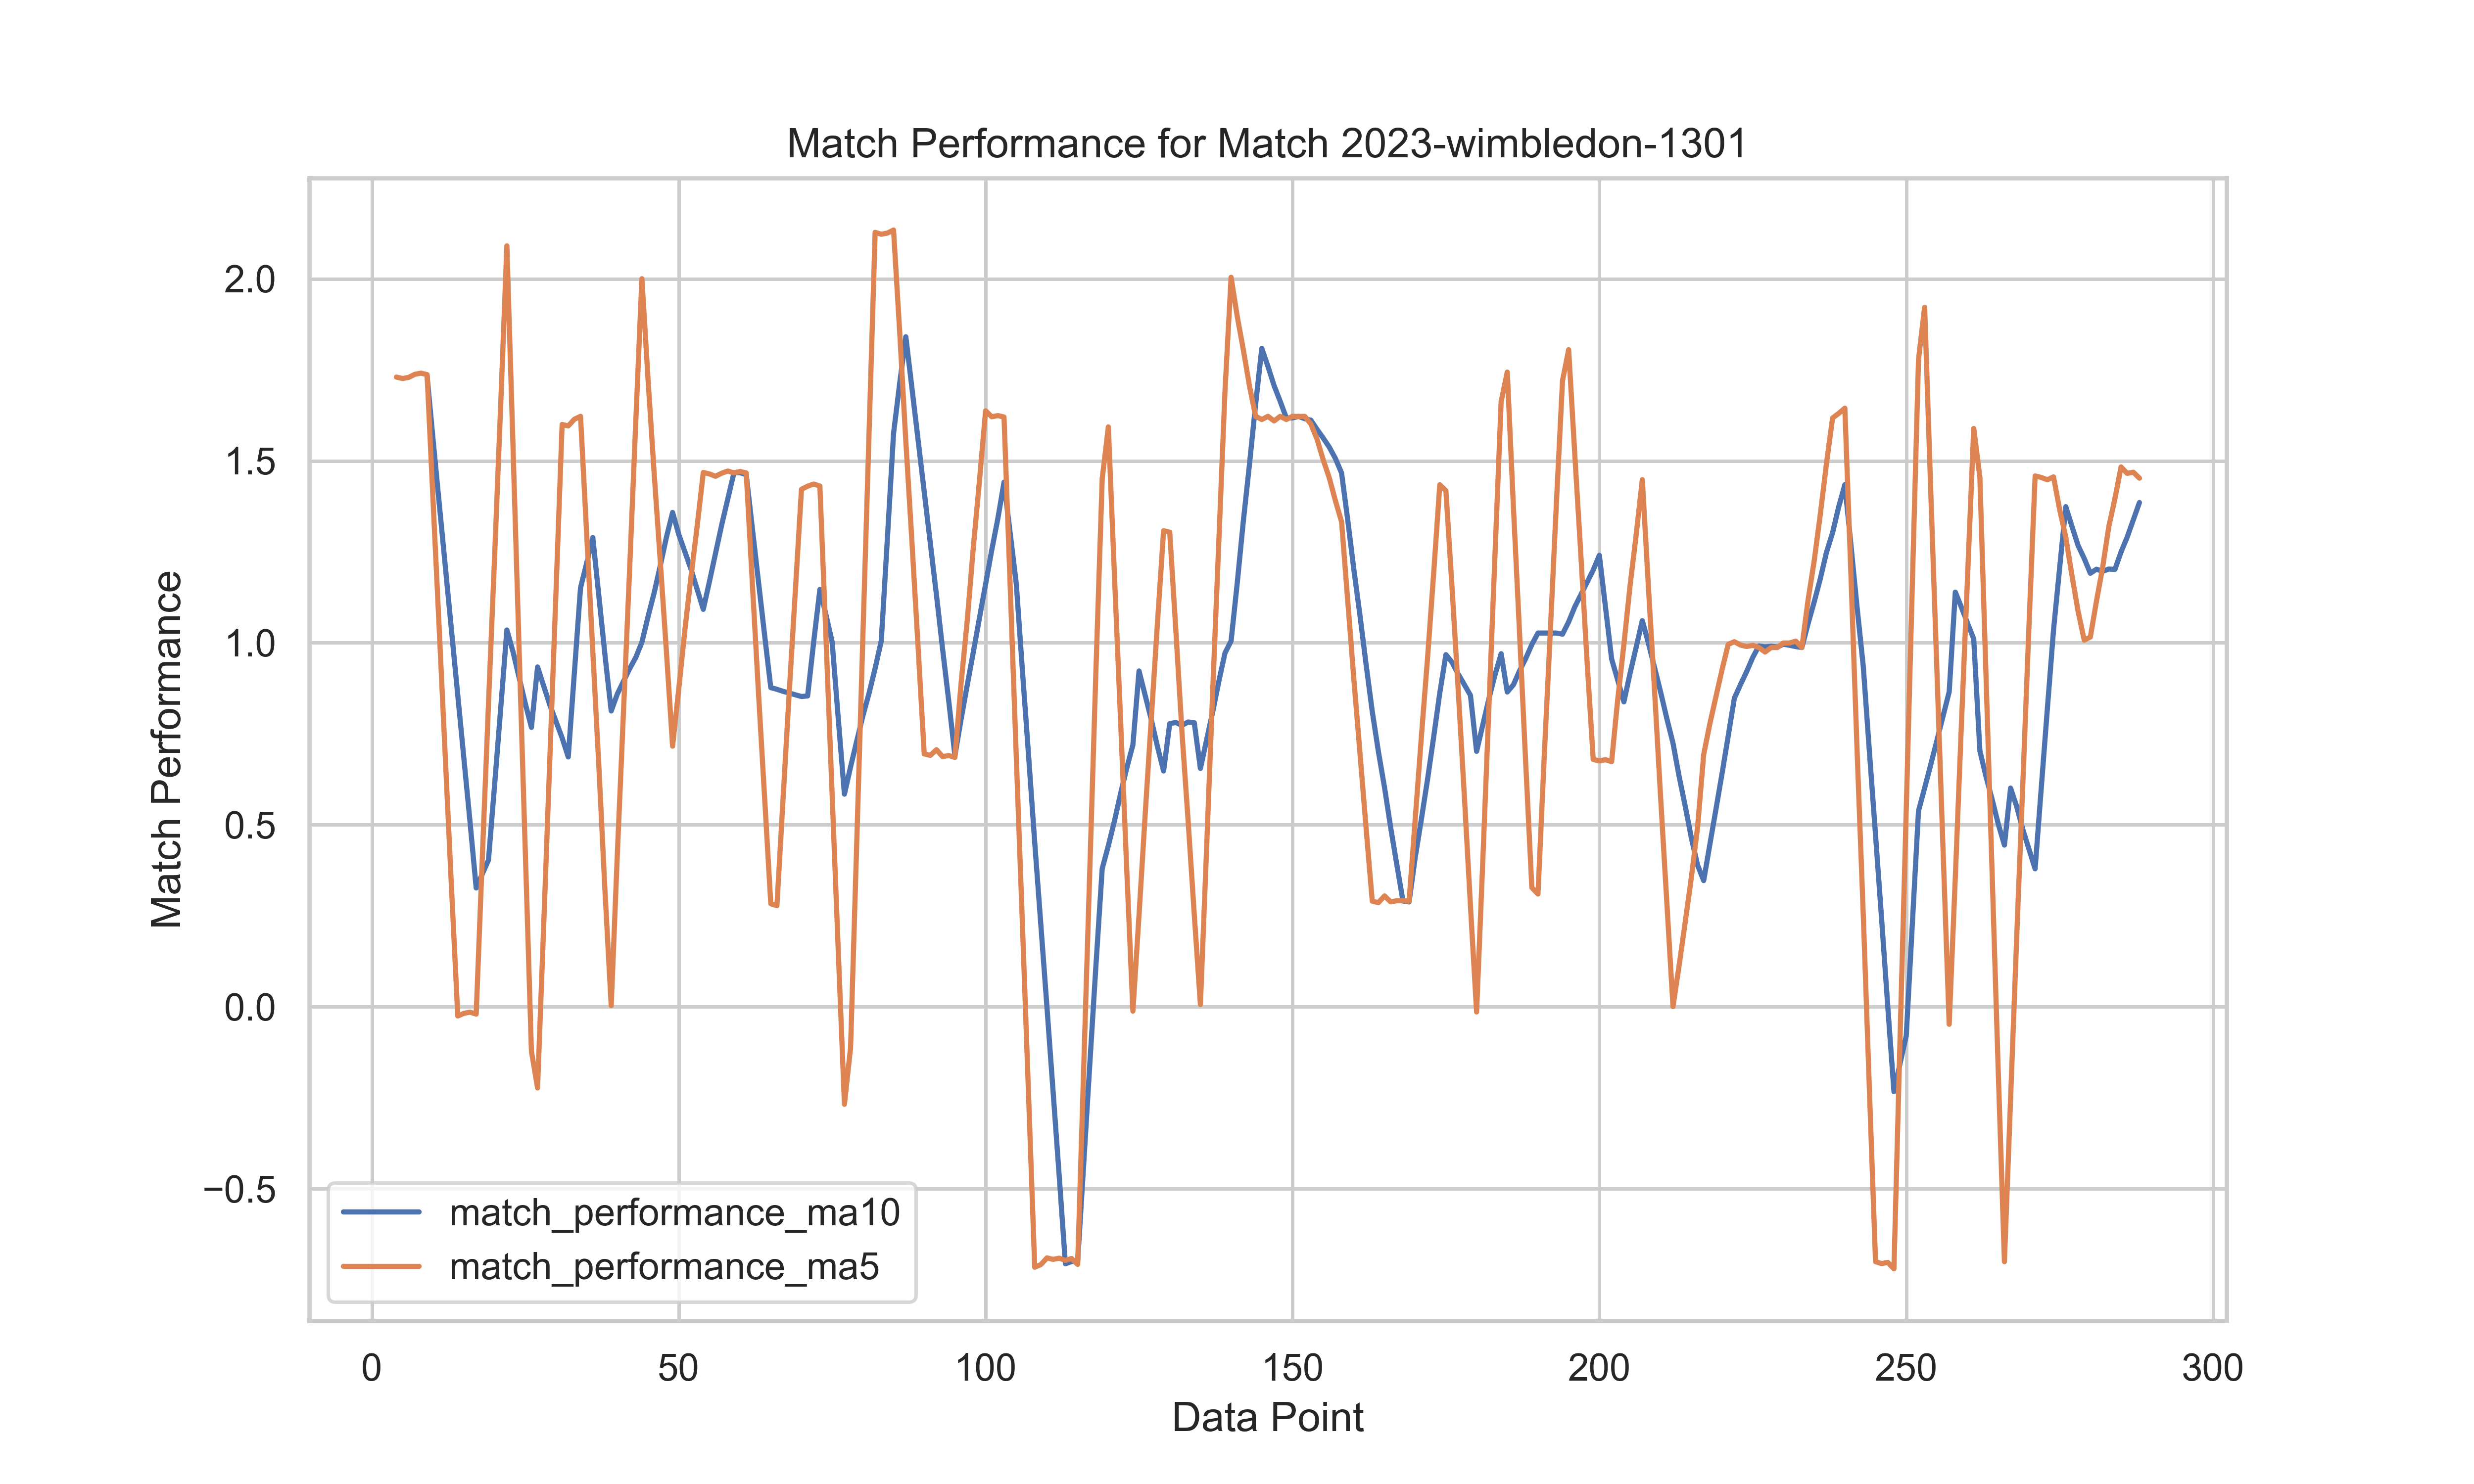
\includegraphics[width=14cm]{match_performance_2023-wimbledon-1301.png}  % 引入图片源
\caption{match performance 2023-wimbledon-1301} \label{fig:match_performance_2023-wimbledon-1301}  % 标题与标签
\end{figure}  % 图片结束

\subsubsection{Accuracy of the model}
\hspace{1.5em}The accuracy of binary logistic regression is 0.6954. This has a good prediction effect for predicting whether a player can score in the actual competition, indicating that this model can evaluate the performance ability of players. However, The accuracy of prediction of gain score is 0.78, and the accuracy of successful prediction of lost score is 0.58.The model prefers to classify samples with label 1.
% 仅包含转折点
\begin{figure}[!htb]  % 图片
\small
\centering  % 居中
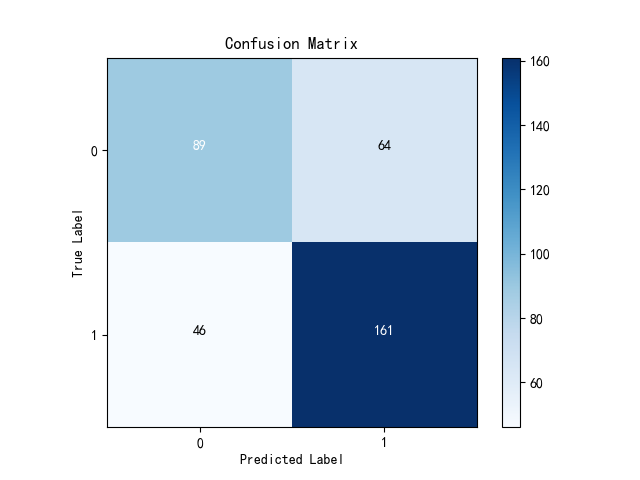
\includegraphics[width=10cm]{Confusion Matrix 1.png}  % 引入图片源
\caption{LR model Confusion Matrix} \label{fig:Confusion Matrix 1.png}  % 标题与标签
\end{figure}  % 图片结束



\subsection{Comparison with other models}
\hspace{1.5em}We also trained other models to compare with logistic regression models.We used Gaussian NB Bayes algorithm for comparison, evaluated auc indicators, and verified with the Five-Fold Cross-Validation. The results are as follows:
ROC diagram shows that LR regression has better effect.

\begin{figure}[!htb]  % 图片
\small
\centering  % 居中
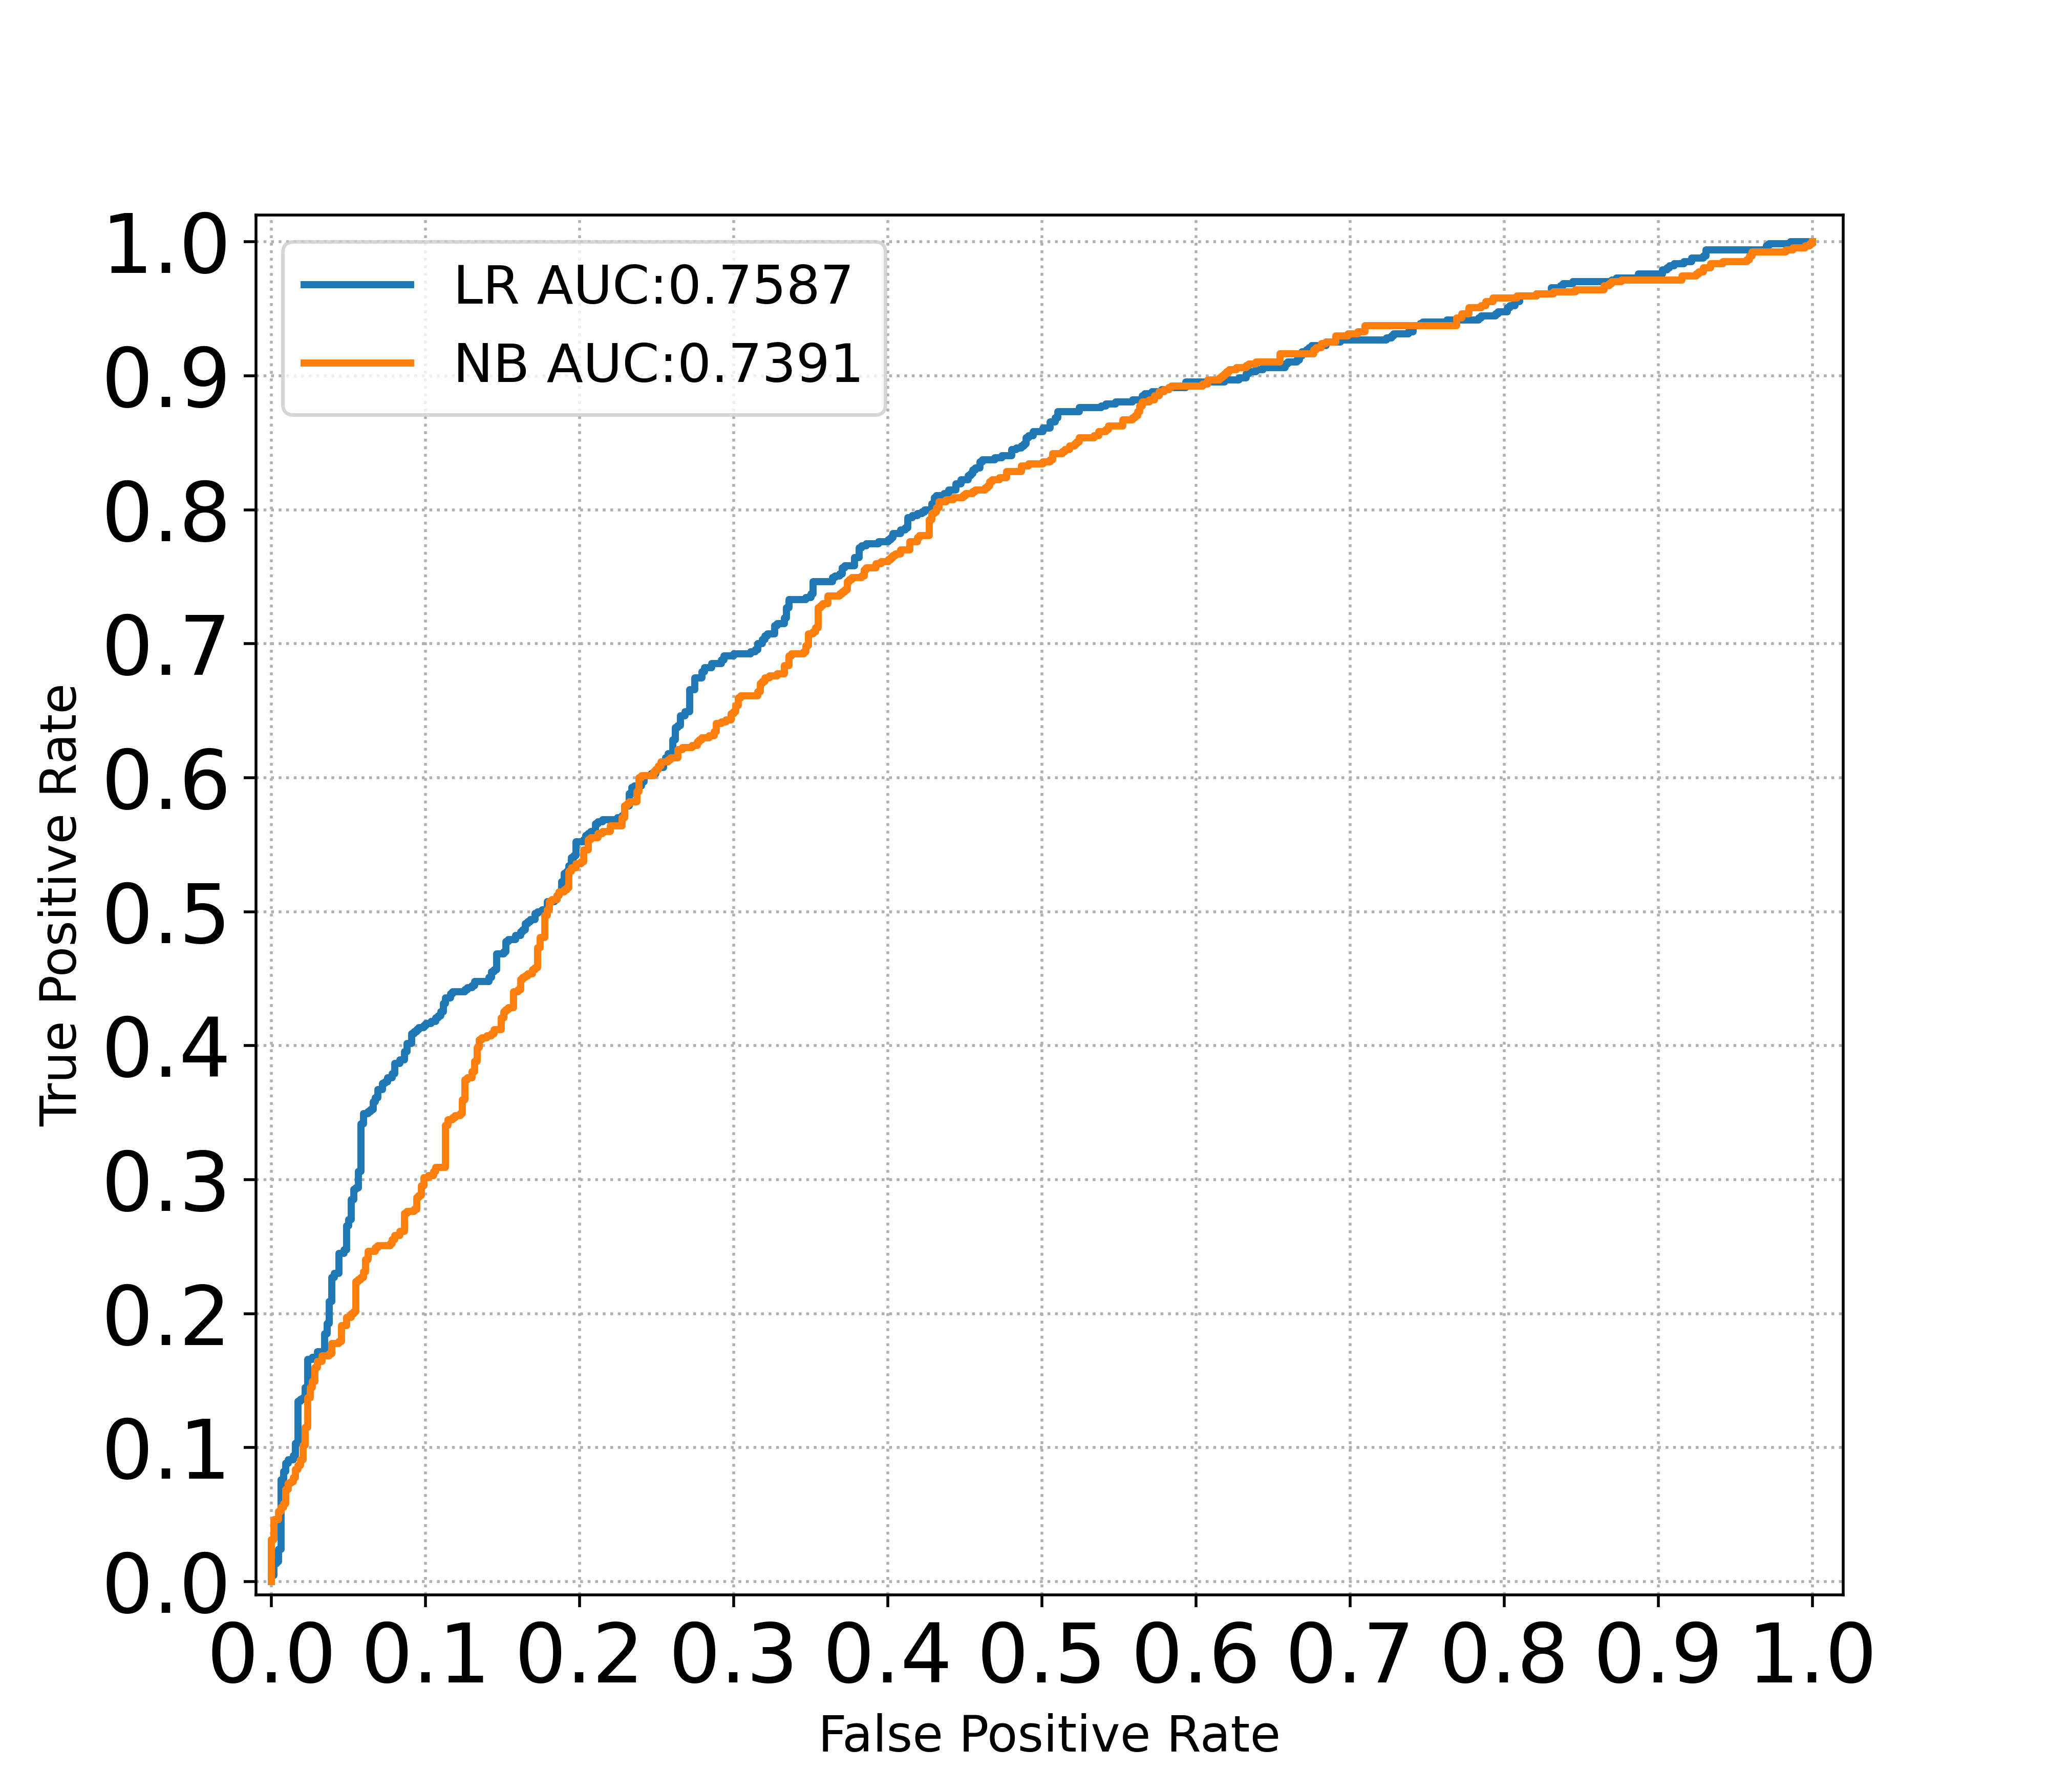
\includegraphics[width=14cm]{问题1_roc_auc(test(采样前)).png}  % 引入图片源
\caption{Comparsion with GaussianNB} \label{fig:Comparsion with GaussianNB}  % 标题与标签
\end{figure}  % 图片结束

\section{Correlation analysis of momentum and victory}
\hspace{1.5em}The coach thinks the players' momentum changes randomly during the game, and the role of momentum in the game is questioned. We will use the knowledge of statistics and visualization to verify the authenticity of the coach's view.

\subsection{Pearson Correlation test}
\hspace{1.5em}\textbf{Null hypothesis (H0):} There is no statistically significant relationship between a player's score in a match and  momentum. 
\par\textbf{Alternative hypothesis (H1):} There is a statistically significant relationship between a player's score in a match and momentum. 
\par\textbf{Significance Level:} We set the significance level at 0.05, that is, we are willing to make the mistake of rejecting the null hypothesis with a probability of 5 percent.
\par The p-value represents the observed correlation coefficient or the probability of more extreme cases occurring,if no linear correlation is assumed between the two variables.
\begin{itemize}
    \item Pearson correlation coefficient: 0.389
    \item  P value: 2.1e-188
\end{itemize}
\par According to the calculated results, the null hypothesis can be rejected, and there is a significant correlation between the quantified momentum data and the score

\subsection{visualization test}

\hspace{1.5em}Visualize the momentum with the score difference between the two players, as 
shown in the figure, and observe that the trend in the figure shows a high degree of similarity. This indicates that the change in momentum is not random, but has a high correlation with how well the players score.

\begin{figure}[!htb]  % 图片
\small
\centering  % 居中
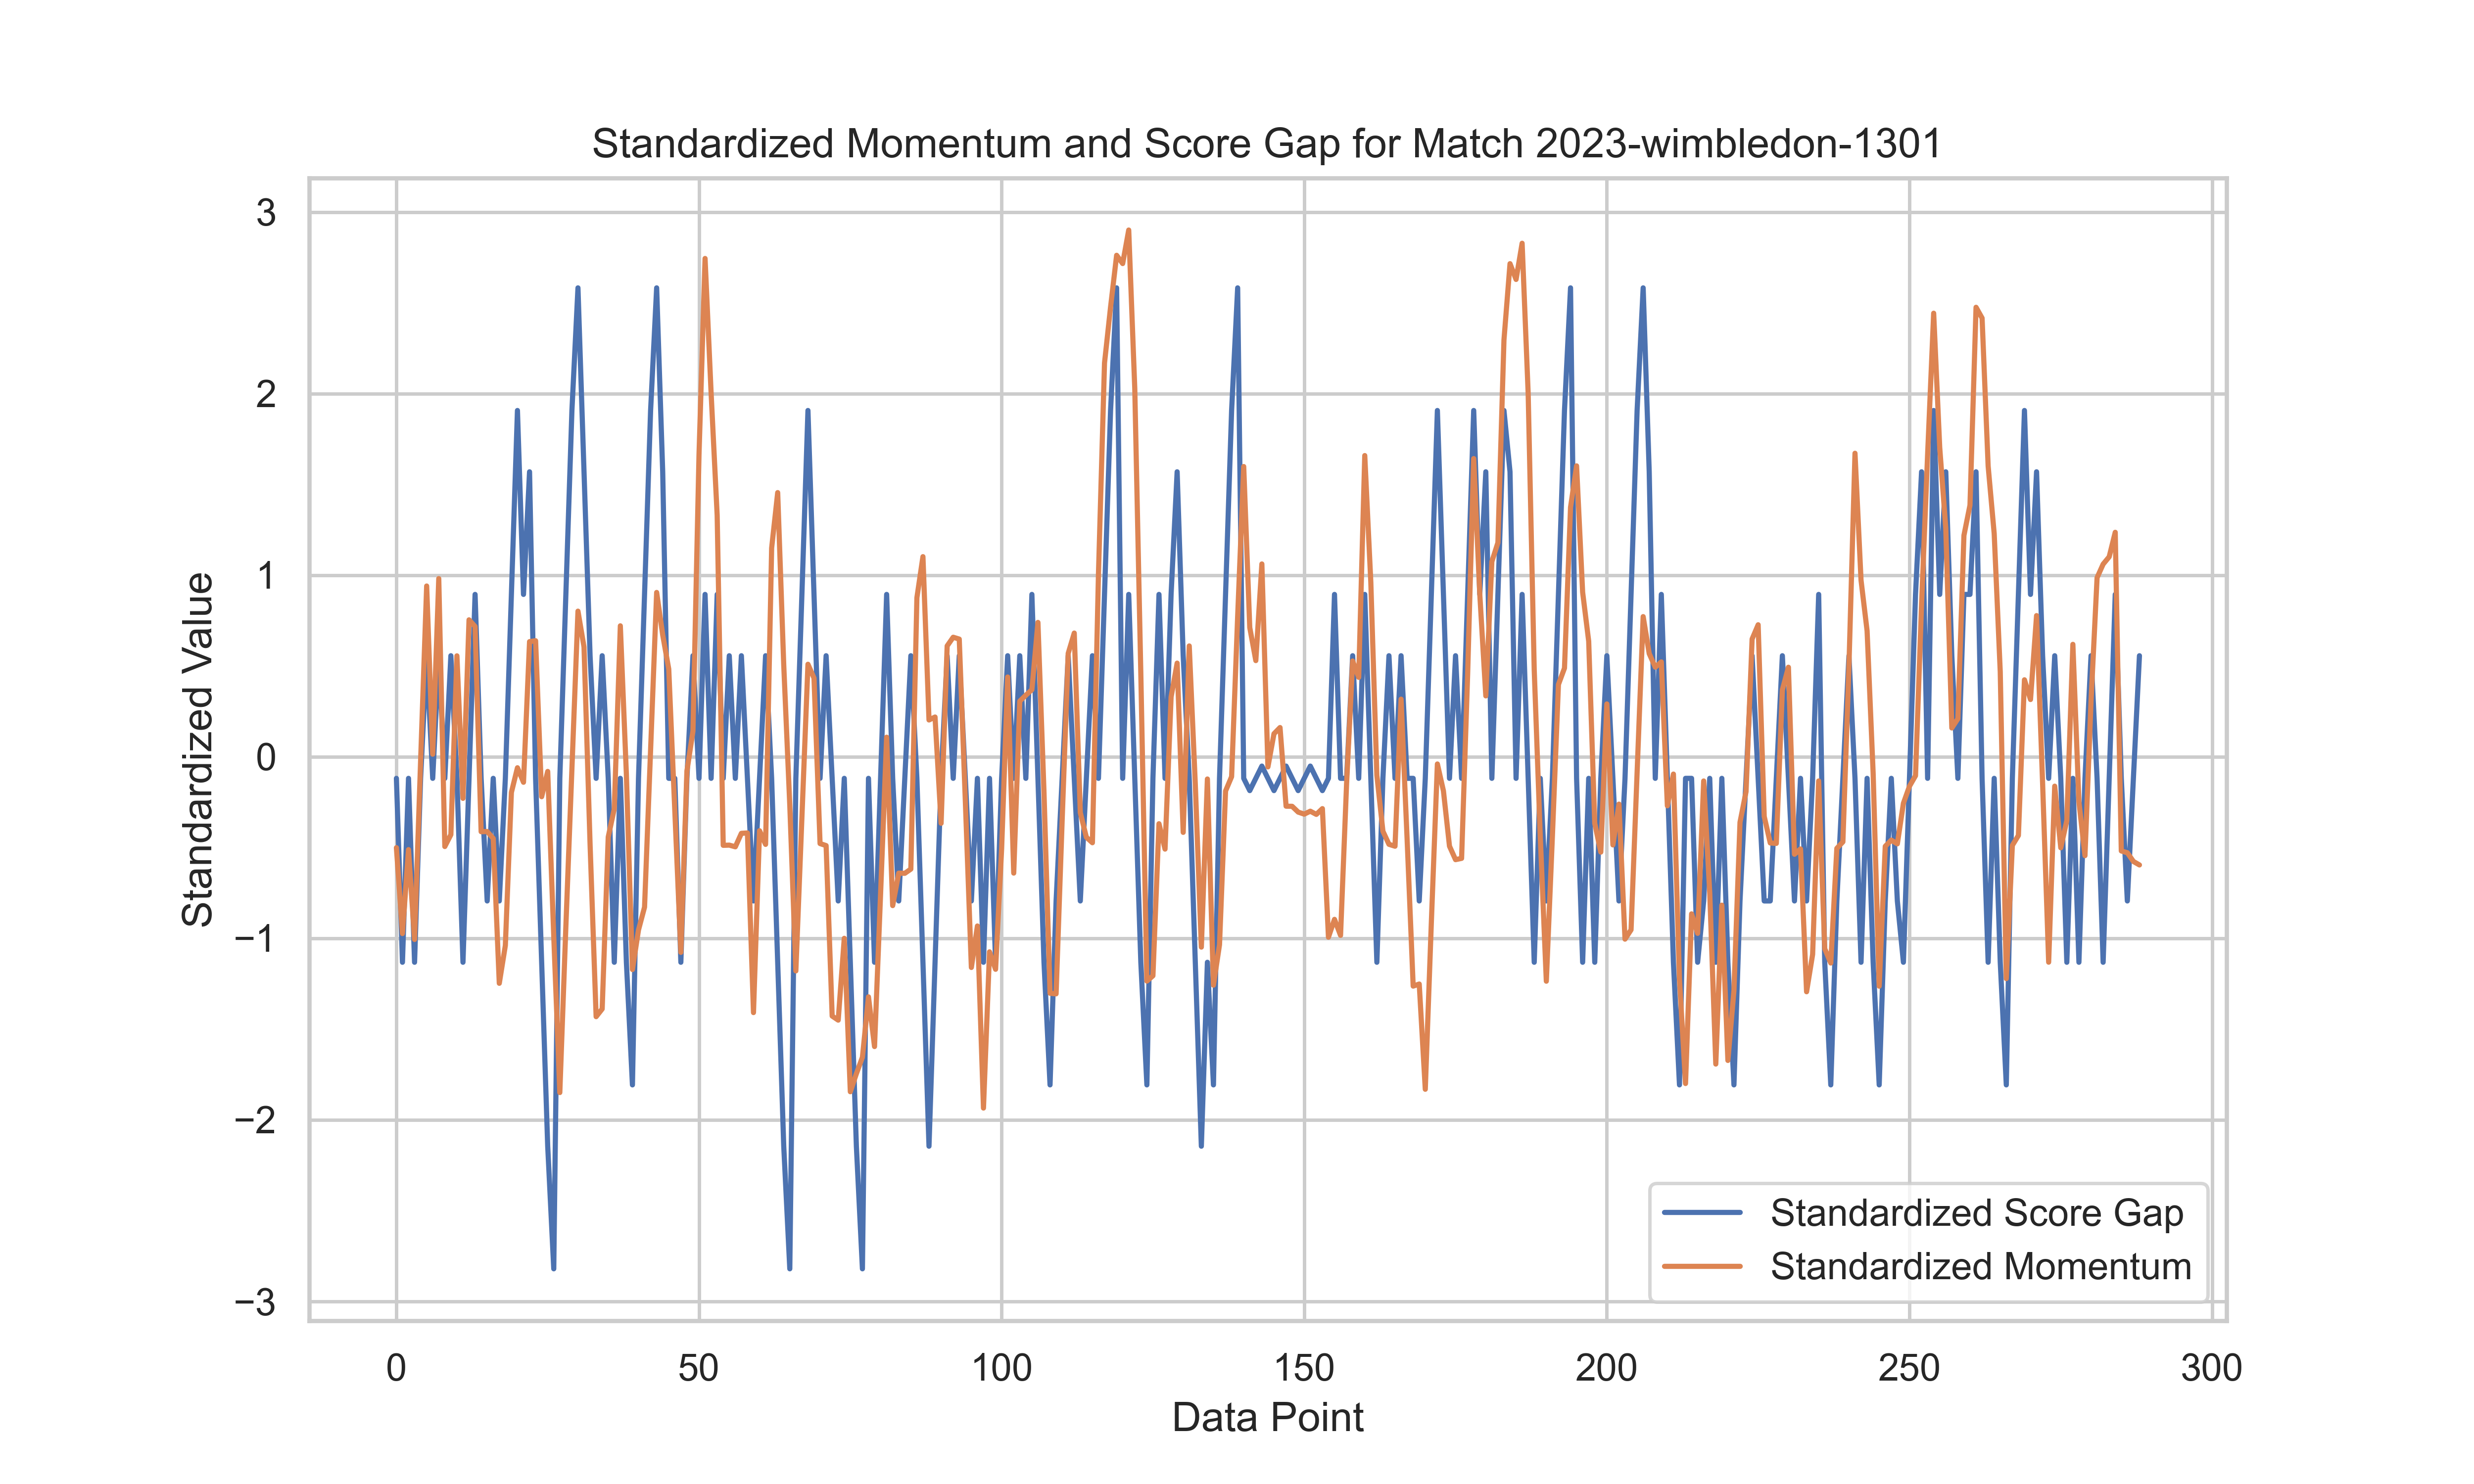
\includegraphics[width=14cm]{standardized_momentum_scoregap_2023-wimbledon-1301.png}  % 引入图片源
\caption{standardized momentum scoregap 2023-wimbledon-1301} \label{fig:standardized_momentum_scoregap_2023-wimbledon-1301.png}  % 标题与标签
\end{figure}  % 图片结束
\newpage
\section{Model \Rmnum{2}:Models to predict the shifts of match trends}

\subsection{Seek  transition points}

\hspace{1.5em} The momentum curve itself is a barometer of the game, which can show that when the situation of the game shifts from one player to another at a certain moment.Thereforemwe define the time when momentum change fast as the transition point. Then the predicted transition points were obtained by random forest model.

% 仅包含转折点
\begin{figure}[!htb]  % 图片
\small
\centering  % 居中
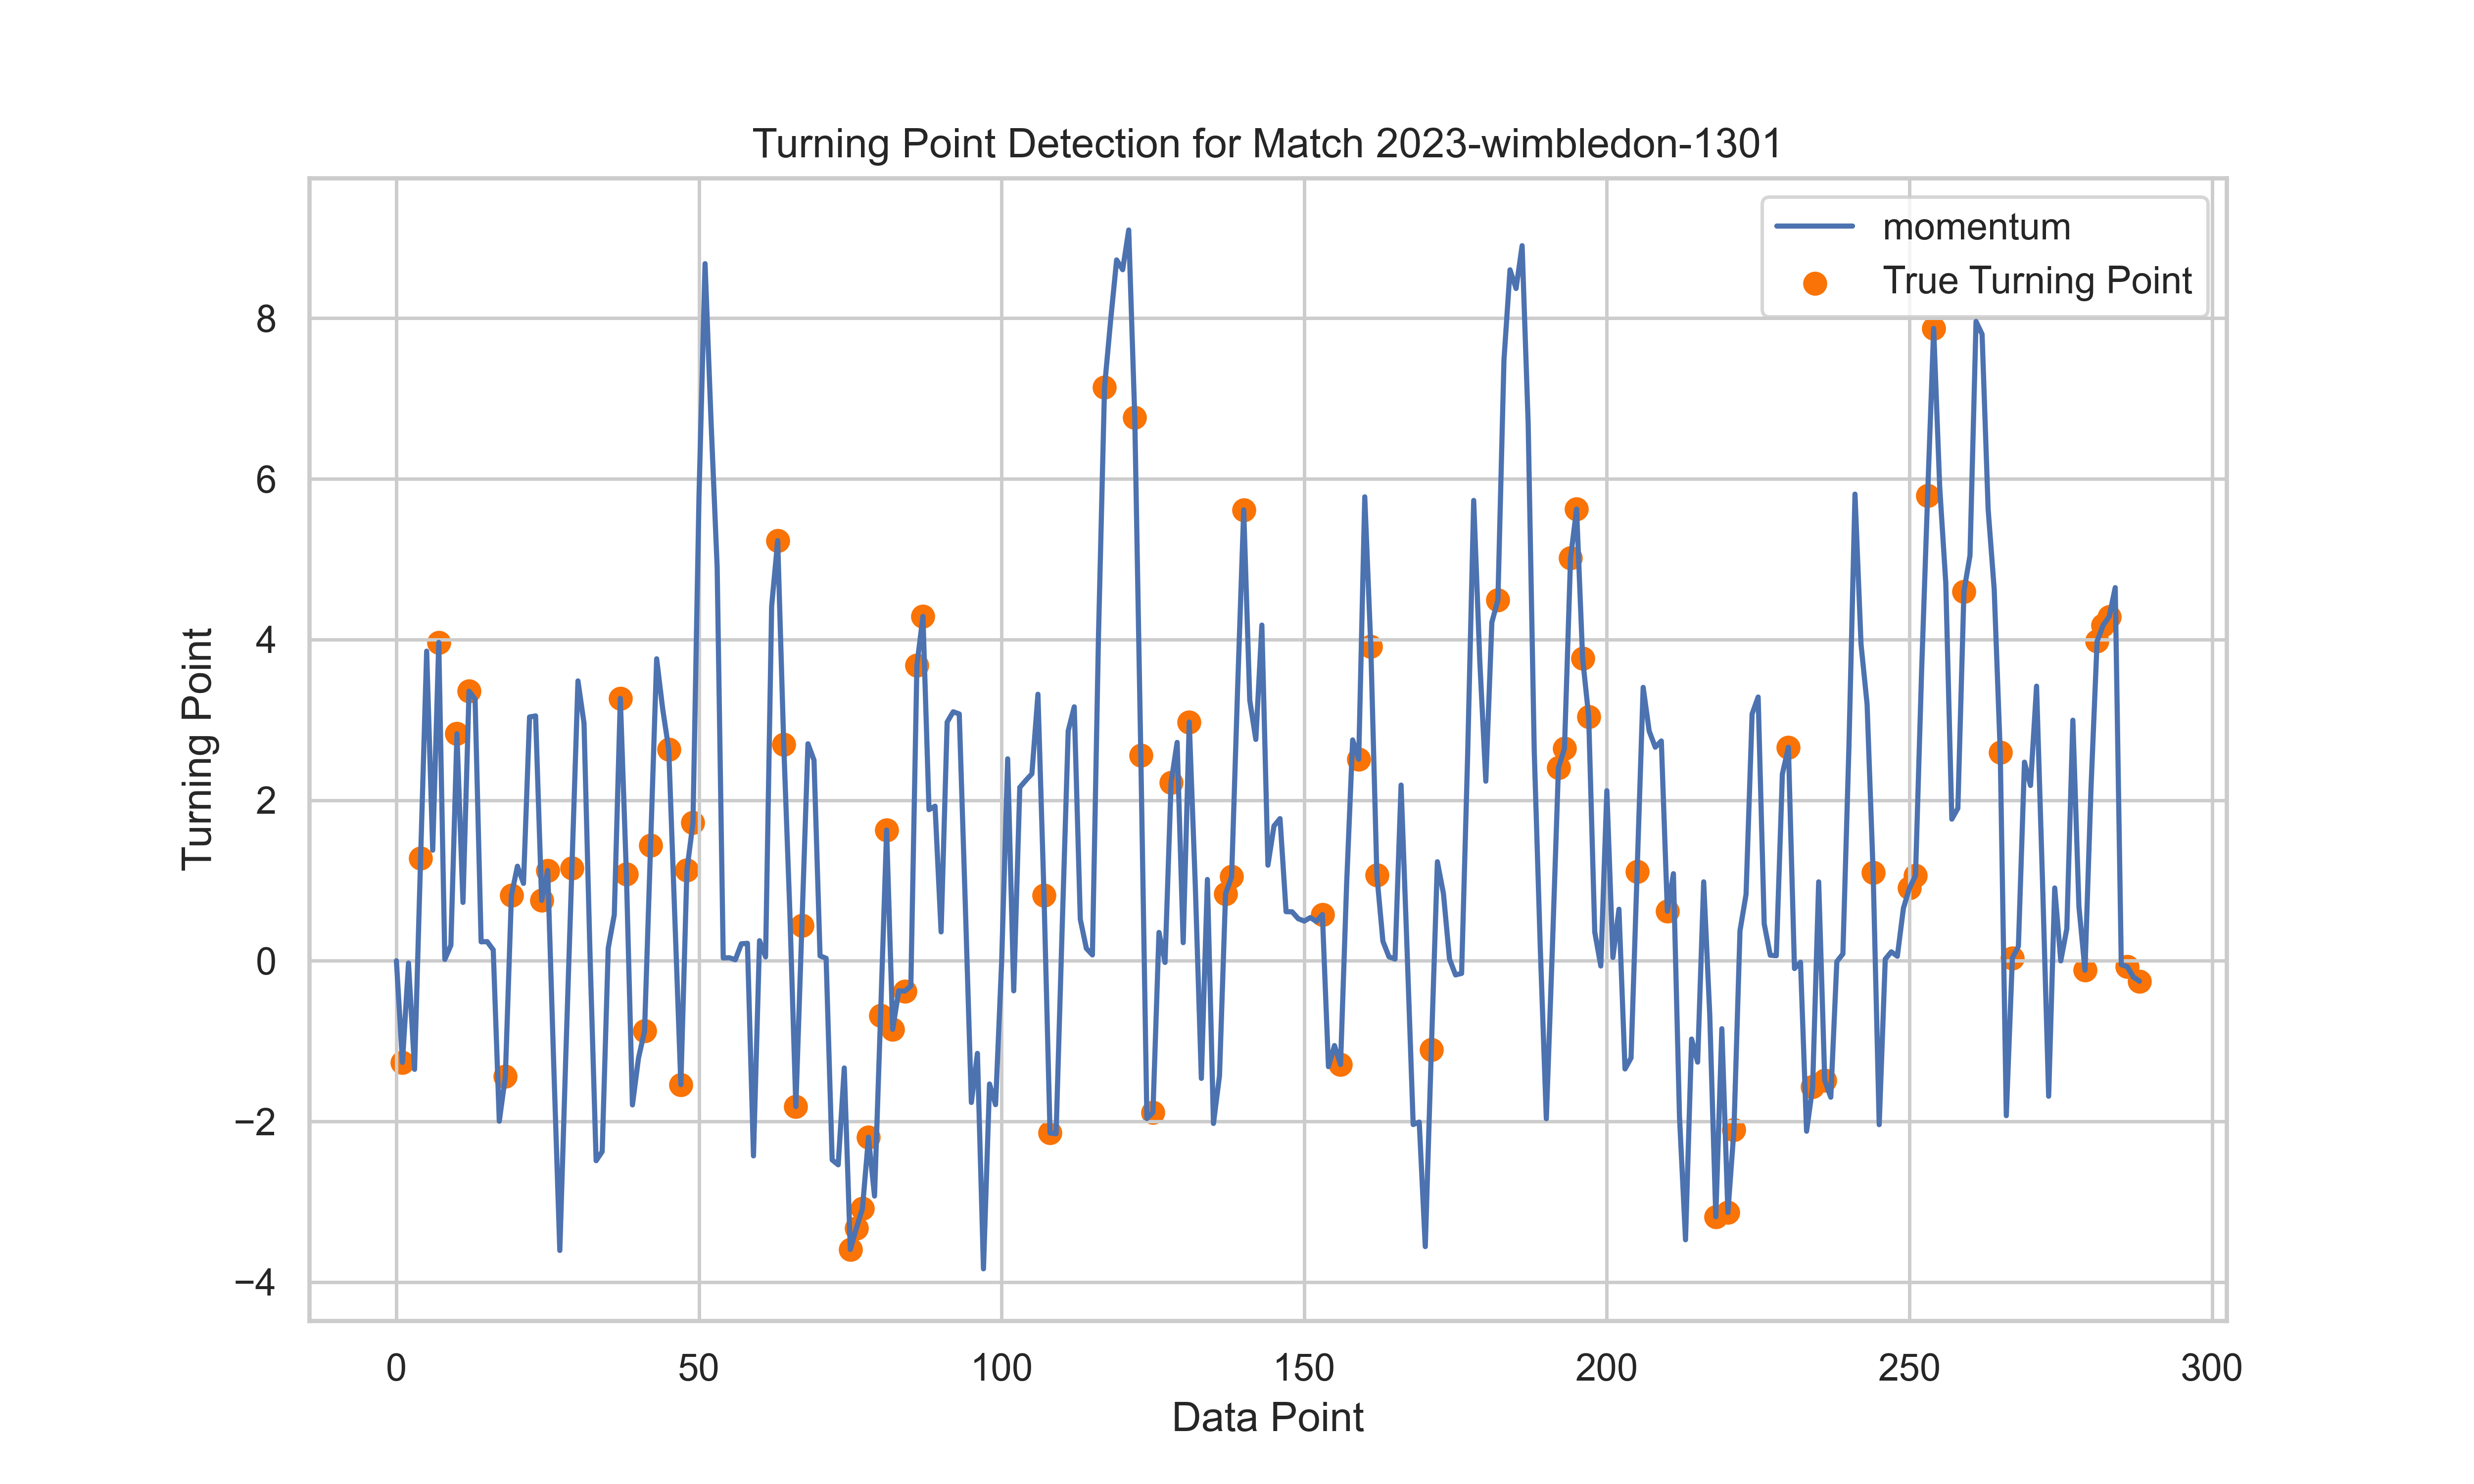
\includegraphics[width=14cm]{turning_point_detection_2023-wimbledon-1301.png}  % 引入图片源
\caption{turning point detection 2023-wimbledon-1301} \label{fig:turning_point_detection_2023-wimbledon-1301.png}  % 标题与标签
\end{figure}  % 图片结束

\subsection{Prediction of transition points by random forest model}

\hspace{1.5em} We use the random forest model for prediction, which is based on the synthesis of multiple decision trees. It is robust to noise and outliers, and can better deal with complex data in real tennis matches. Second, our data contains multiple features, and random forests can efficiently process high-dimensional data without the need for feature selection. Finally, the Random Forest provides a ranking of the importance of each feature, indicating which features are most influential in predicting turning points.
\par We create a random forest classification with 100 decision trees, divide the data set into a training set and a test set, train the model on the training set, make predictions on the test set, and calculate the model performance index.
\par Next, we visualized prediction results,marking the real turning point and the predicted turning point.

\begin{figure}[!htb]  % 图片
\small
\centering  % 居中
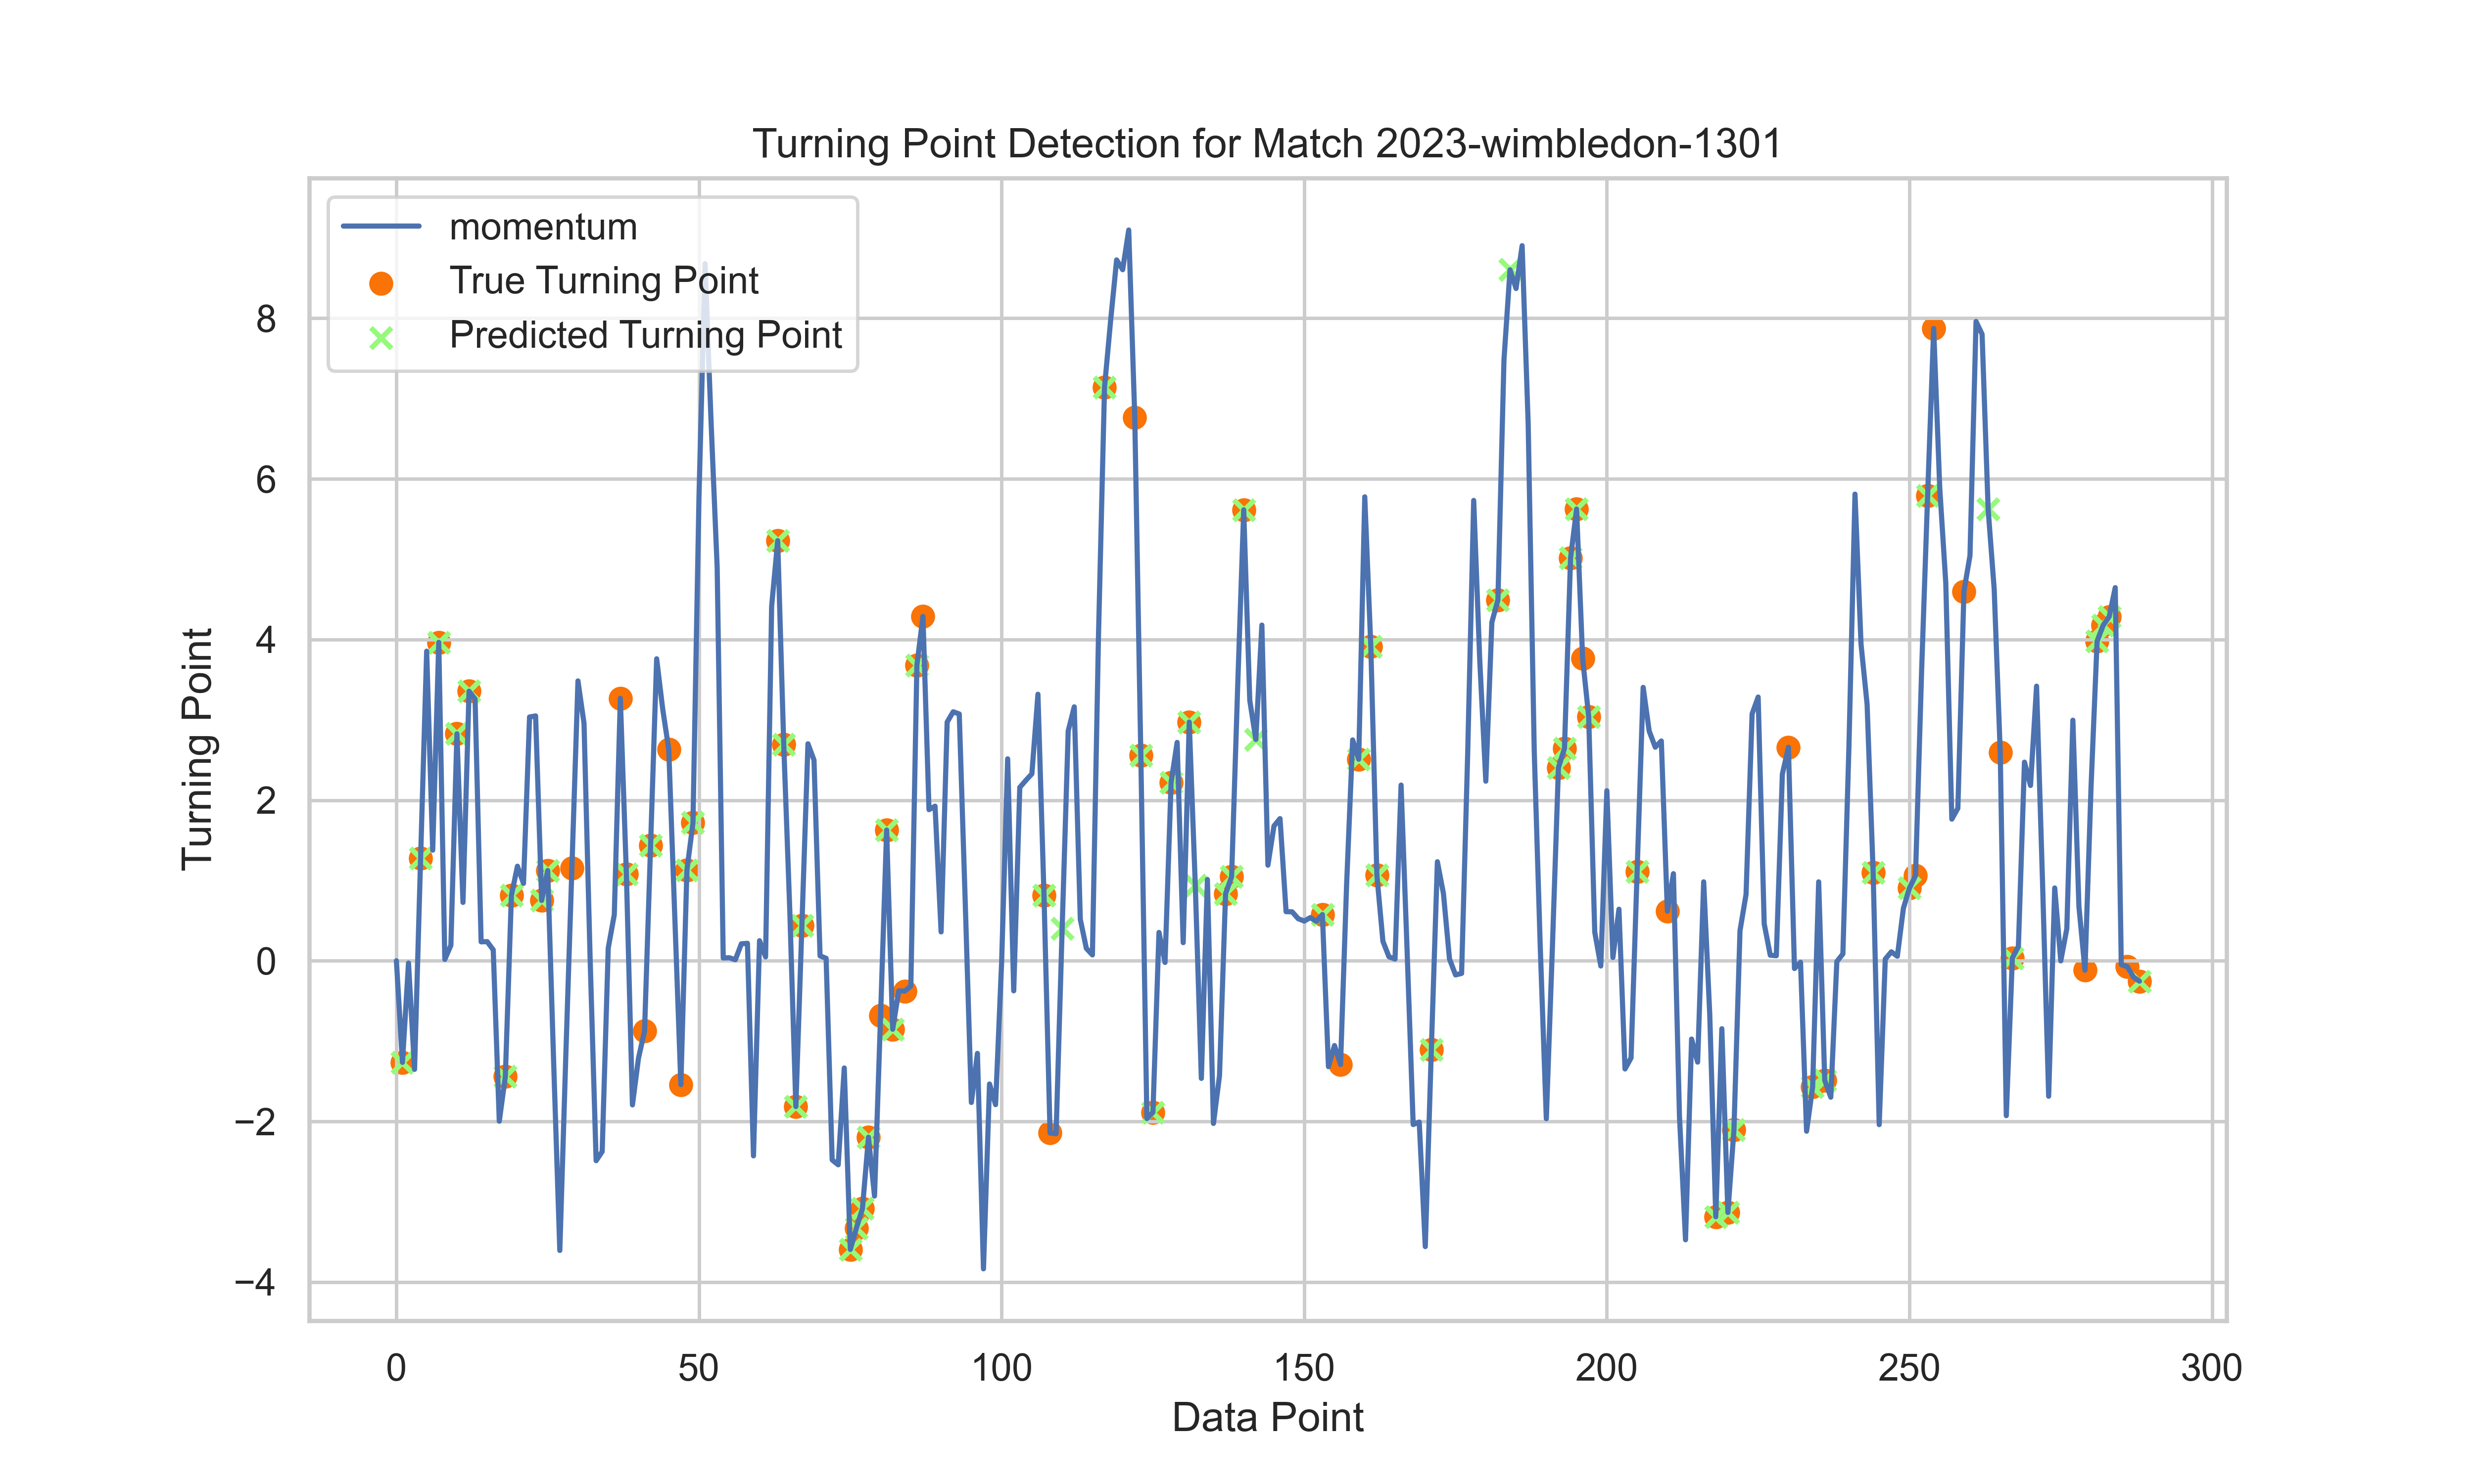
\includegraphics[width=14cm]{turning_point_detection_2023-wimbledon-1301_prediction.png}  % 引入图片源
\caption{turning point detection 2023-wimbledon-1301 prediction} \label{fig:turning_point_detection_2023-wimbledon-1301_prediction.png}  % 标题与标签
\end{figure}  % 图片结束


\newpage
\subsection{The importance of factors affecting the transition points}
\hspace{1.5em}After the specific moment of situation transformation is obtained from the original data, the importance of each indicator  can be ranked in the current time period, and the indicator with the greatest correlation (positive correlation or negative correlation) is the indicator with the greatest impact on the situation.
\par Output the importance of 10 variables in the random forest model. From the figure below, we can see that X8, the total chart run distance within the last three points, has the greatest influence on the transition point. The score of X1 ,the extent of lead score also influcence a lot .Other factors have few importance.
\newpage
% 对全比赛的图

\begin{figure}[h]  % 图片
\small
\centering  % 居中
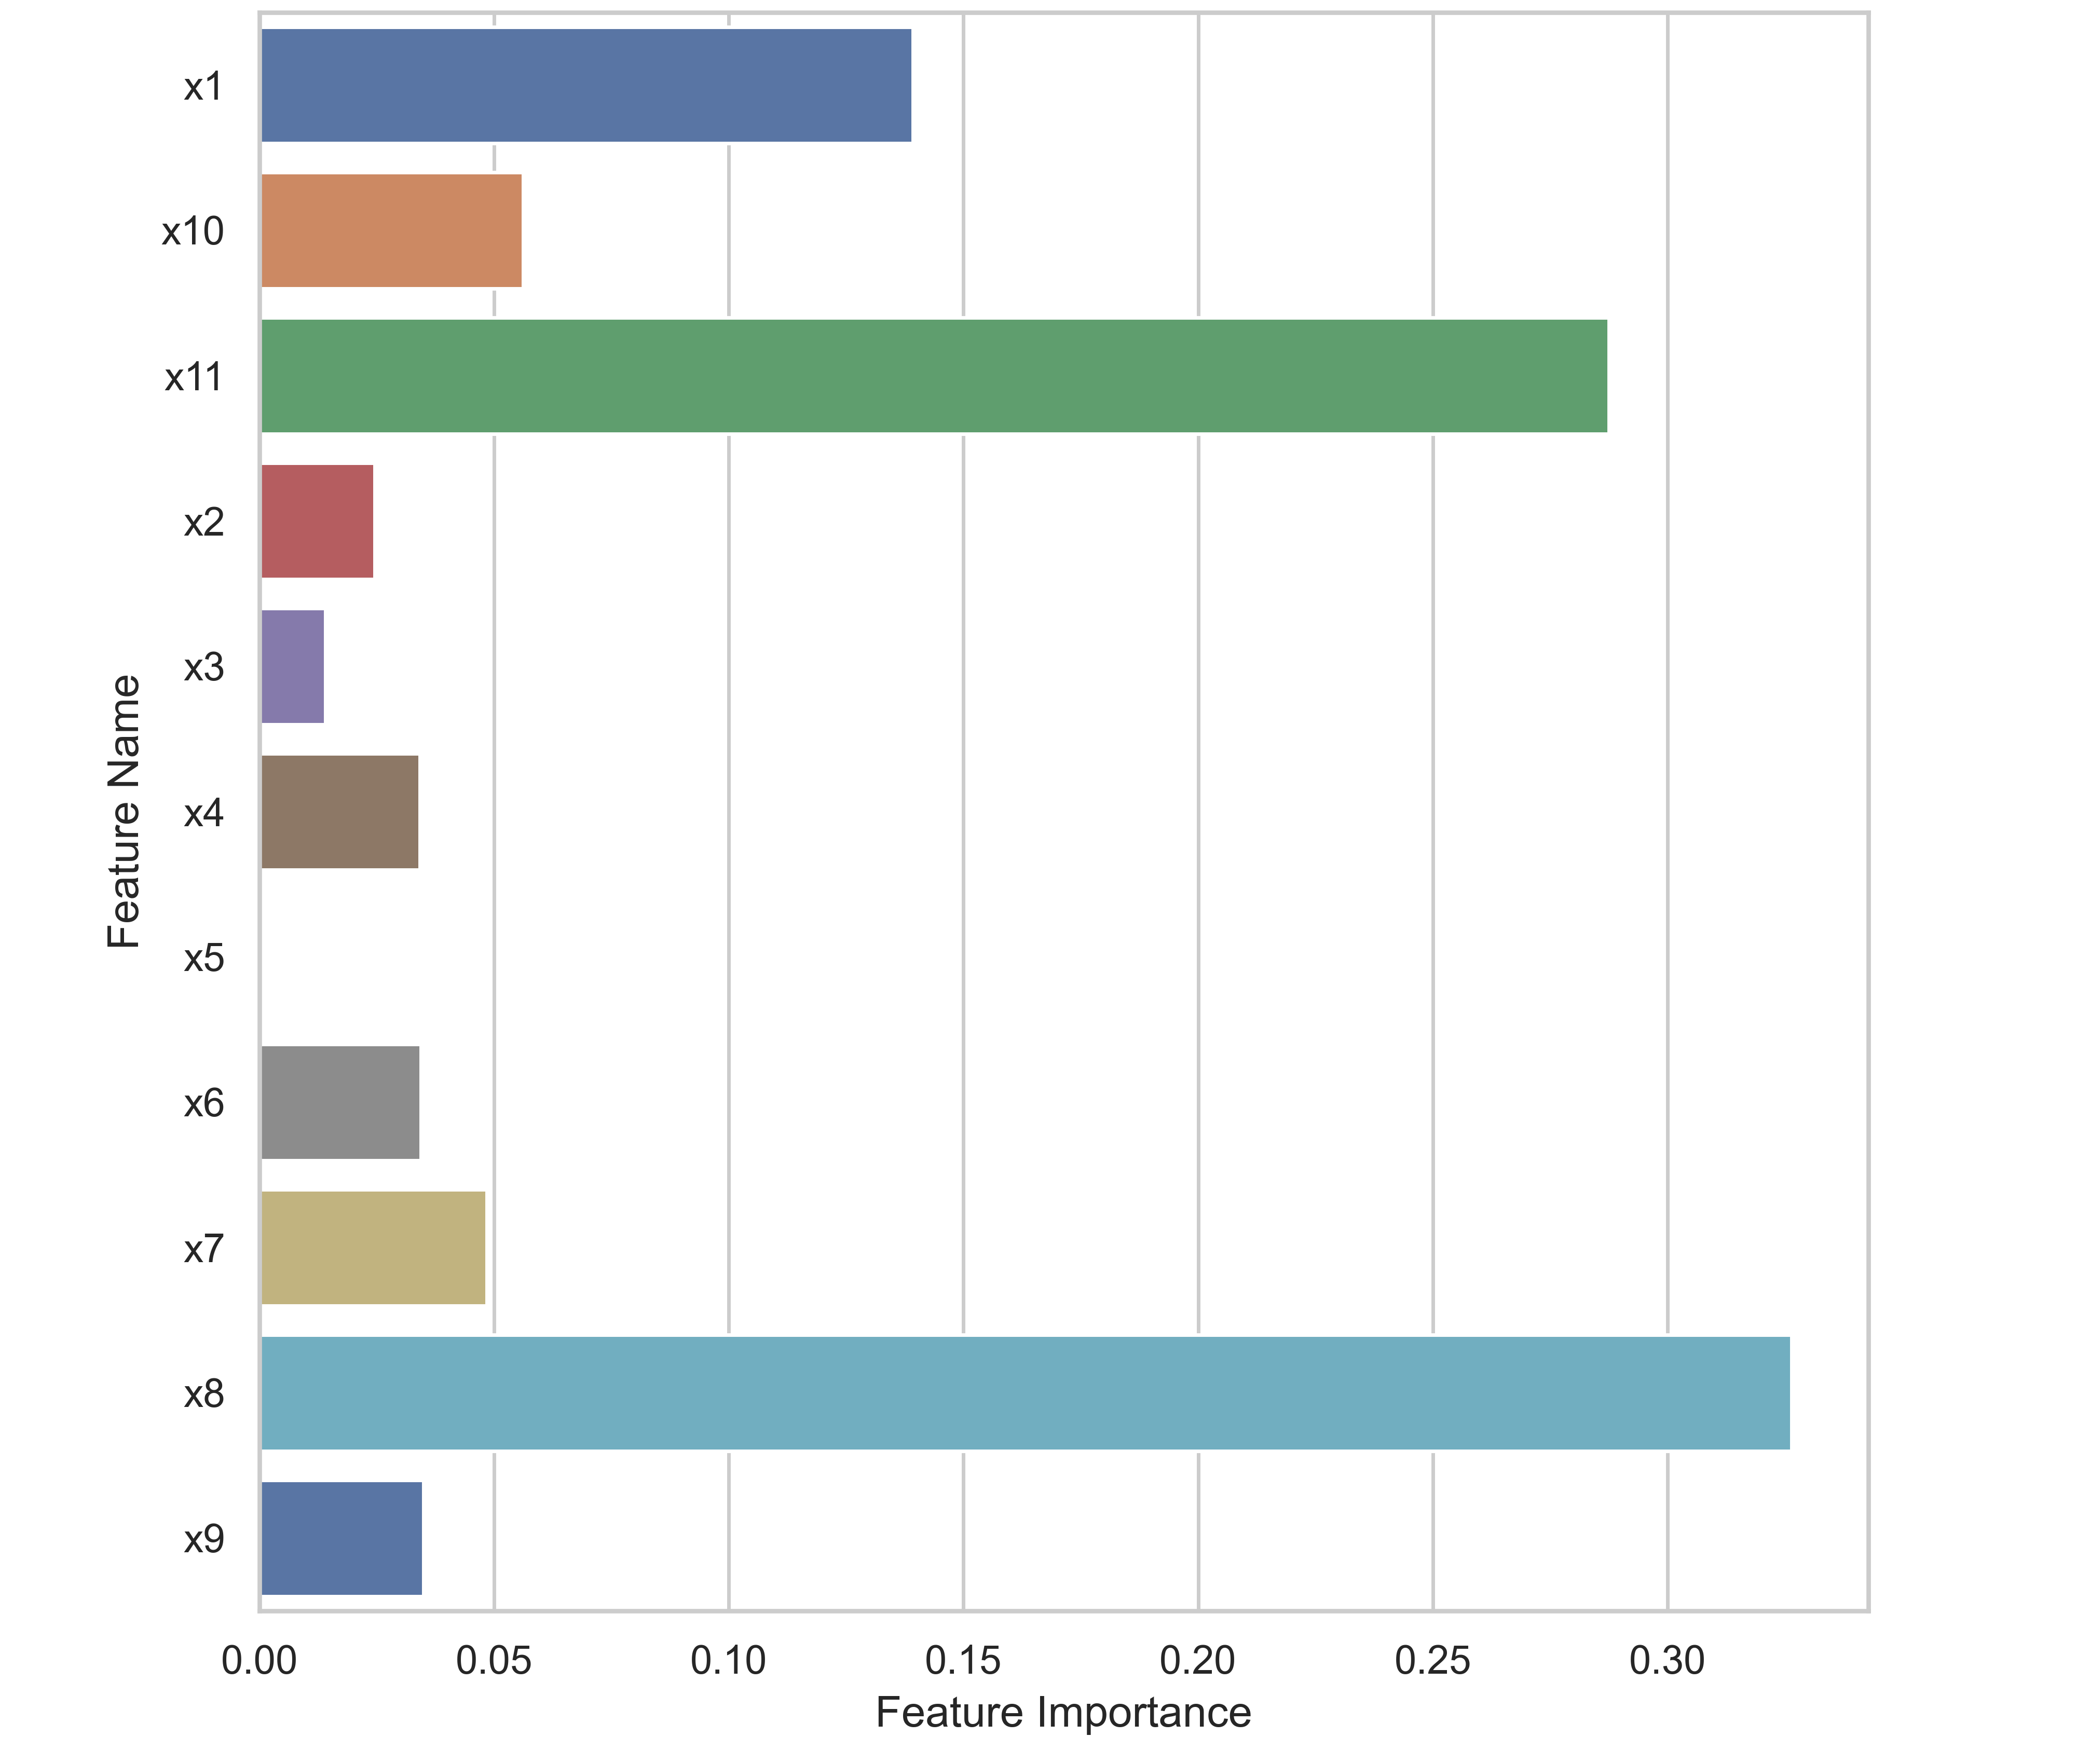
\includegraphics[width=12cm]{feature_importance_1301.png}  % 引入图片源
\caption{feature importance} \label{fig:feature_importance_1301.png}  % 标题与标签
\end{figure}  % 图片结束

% This is Figure \eqref{fig:turning_point_detection_2023-wimbledon-1301_prediction.png}.  % 引用图表
% % This is table 1 \eqref{tab1}
% % This is table 2 \ref{tab2}

% Feature,Importance
% x1,-0.0023725385064628838
% x2,0.04564500947833025
% x3,0.10486219883746727
% x4,0.7017356104151932
% x5,0.0
% x6,-0.6906612523309515
% x7,0.3028275197256524
% x8,0.00021046352080887008
% x9,1.3214960009582046
% x10,-0.06230170308017339

\subsection{Advise players on transition points}
\subsubsection{General recommendations}
\hspace{1.5em}The above analysis shows that the running distance is highly correlated and greatly affects the turning point of the situation. In other words, physical exertion is very important in tennis matches.Players should mobilizing the opponent running distance as much as possible.They should reduce their own running distance,such as constantly switch the near and far ball, left and right ball, in order to retain their own physical strength, consume the opponent's physical strength. 

\subsubsection{Separate recommendations for specific players}
Take  Novak Djokovic as an example, we put the data of several matches into the model, obtained the importance of each factor, and found that X8,X11, both running distance and whether it is the service game are the key factors, indicating that the player has a high serving ability, and when facing this player's service game, we should be mentally prepared and alert.
\begin{figure}[!htb]  % 图片
\small
\centering  % 居中
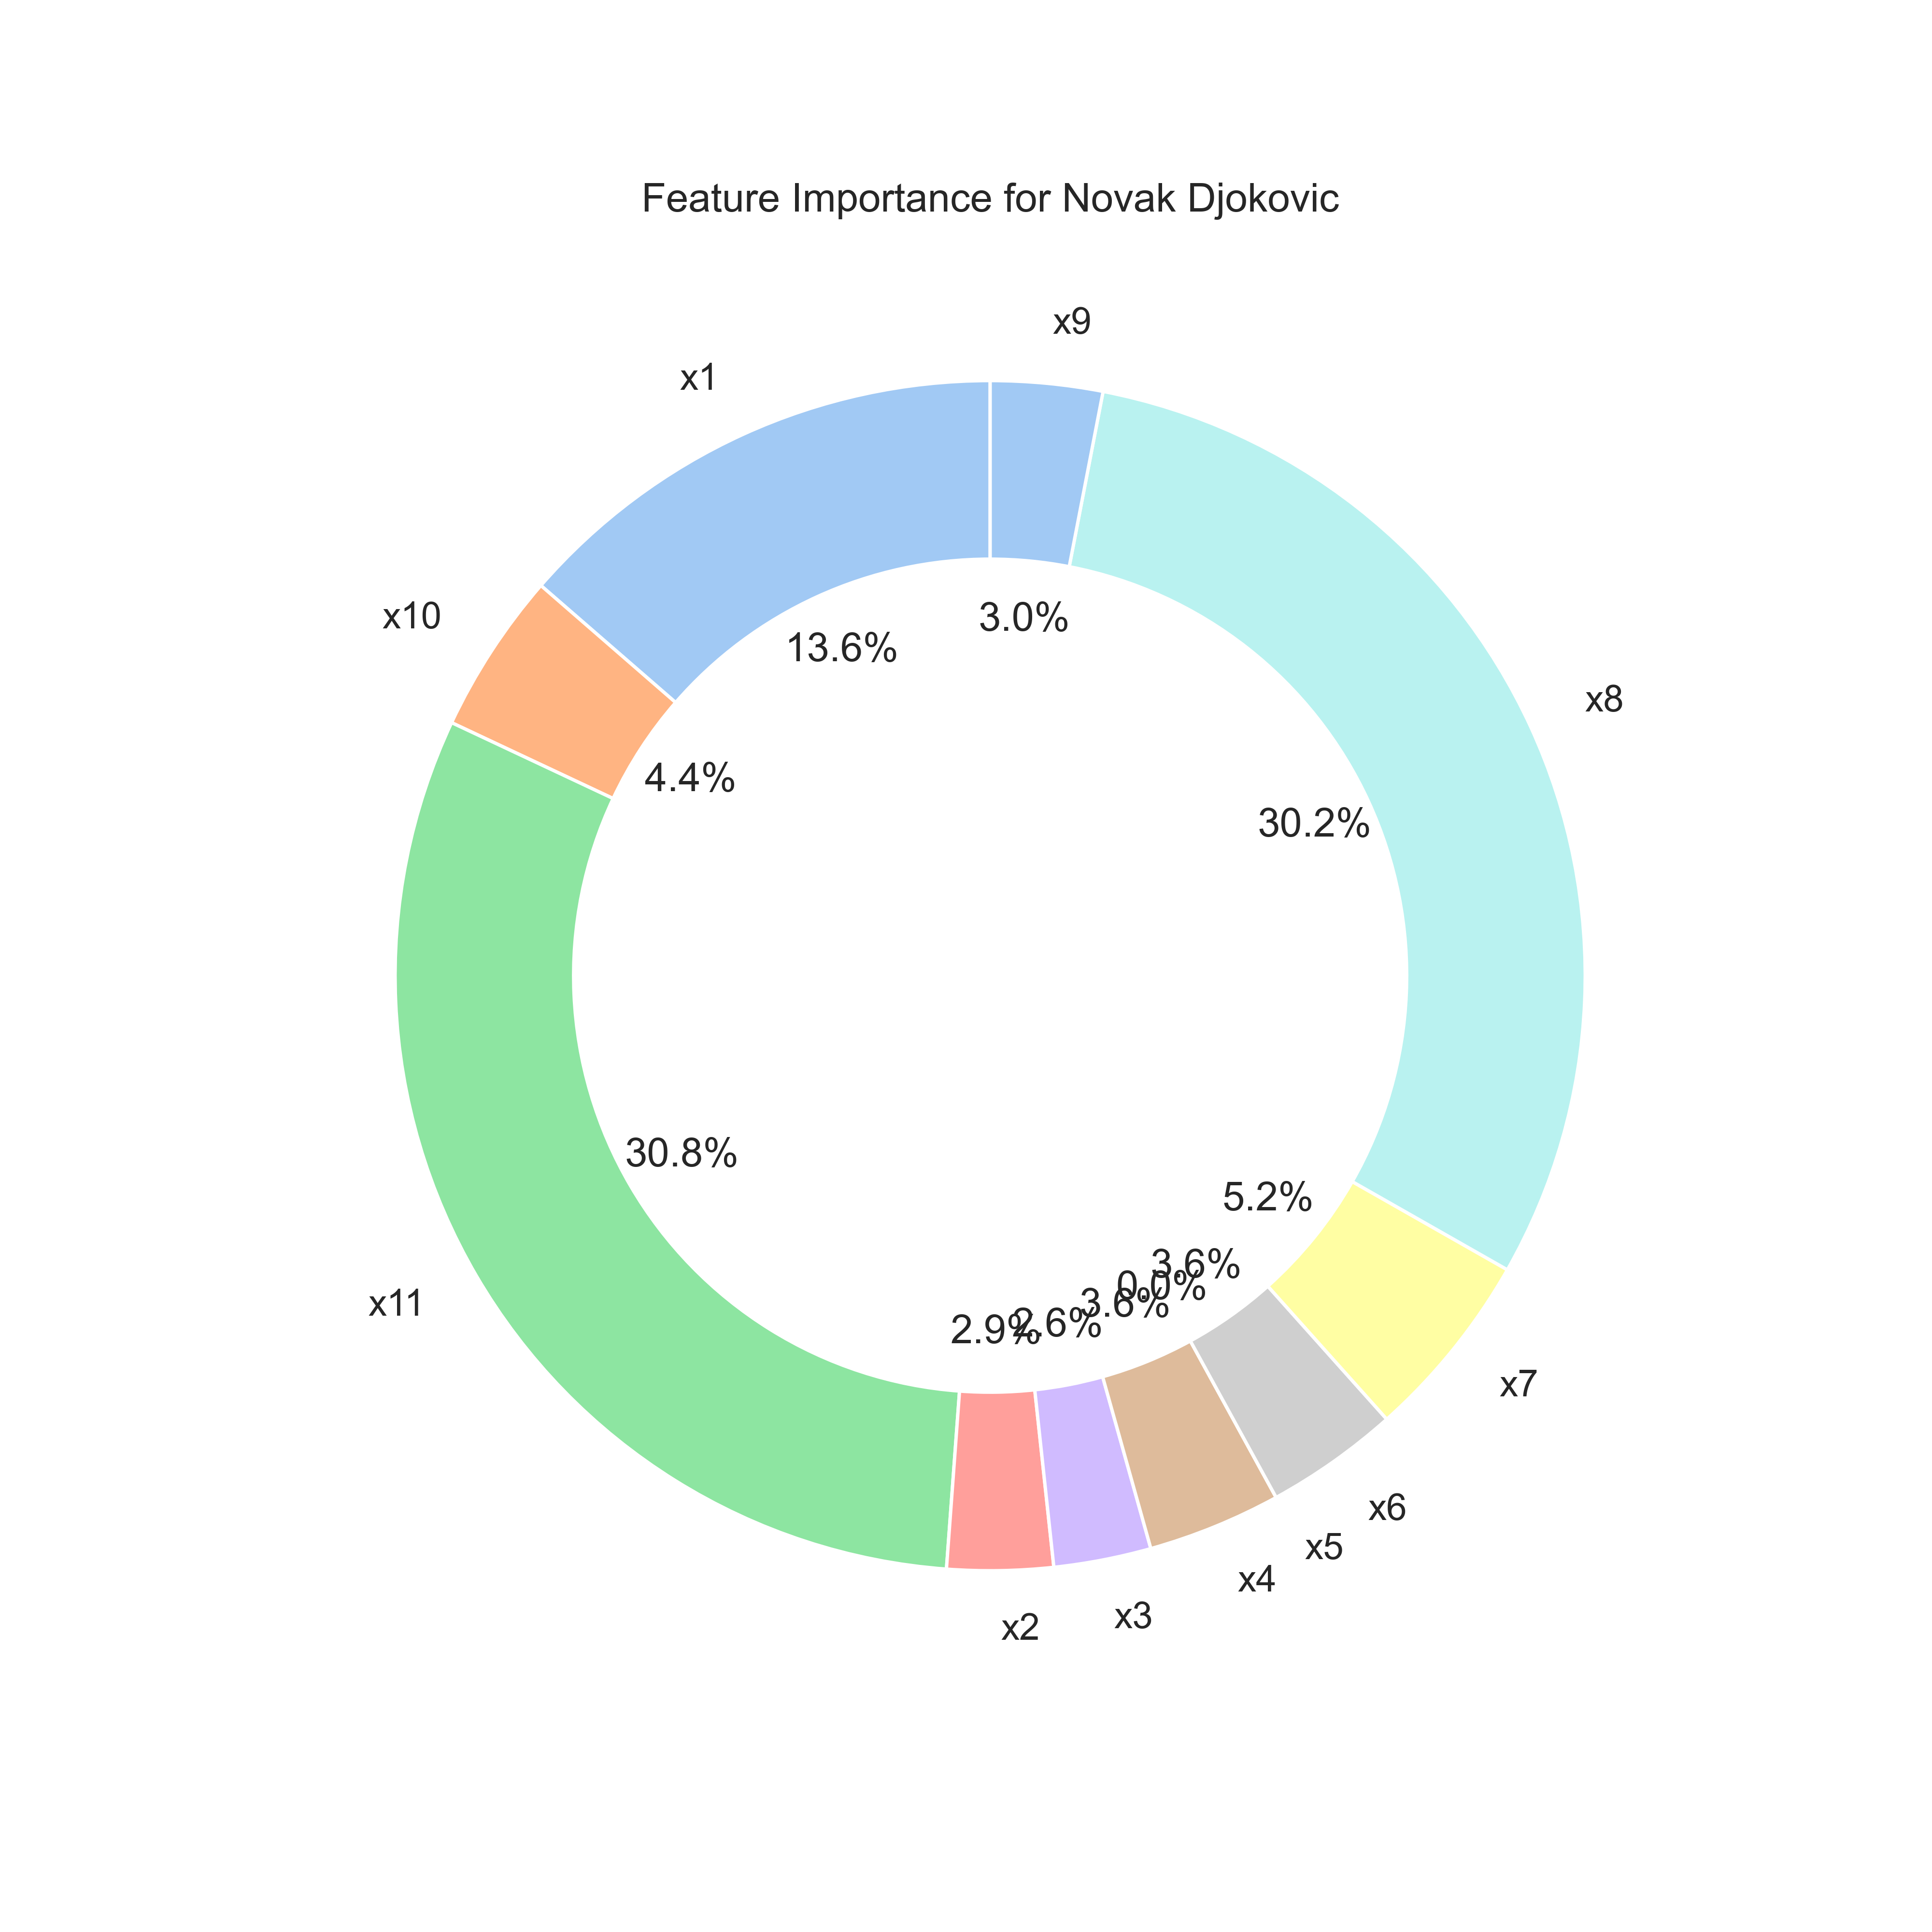
\includegraphics[width=11cm]{feature_importance_Novak Djokovic.png}  % 引入图片源
\caption{feature importance Novak Djokovic} \label{fig:feature_importance_Novak Djokovic.png}  % 标题与标签
\end{figure}  % 图片结束



\section{Model generalization evaluation}

\subsection{Application of the model to other matches}

\hspace{1.5em}We have completed the model of transition points in the competition, and the prediction result is good. Next, we continue to test the random forest model of Question 3 on other data sets to check the generalization ability of the model.
\hspace{1.5em}We used the random forest model to predict the male/female single data set, and the prediction effect of the model is as follows
%Women's singles
\hspace{1.5em}It can be seen that the model performs well on other data sets and can be applied to tennis match prediction
\hspace{1.5em}
Below is the Model accuracy index:\\
Women's singles : 0.683\\
men's singles : 0.718



\subsection{Application of the model to other sports}  % 一级标题
\hspace{1.5em}Our model is based on the analysis of tennis data, some of which, such as break rate and other indicators, may not exist in other sports. Therefore, we believe that when the model is applied to basketball and other fields, variables can be modified as follows:
\par In terms of basketball, we need to change the scoring system due to a single shot within basketball that is equivalent to a point in tennis can have the result of 1(ex: free throw),2(shot scored within 3-point arc),or 3 points(shot scored outside of 3-point arc). Also rules regarding fouls and penalties are also diverse from tennis and complex in its own way, making us including more rules within the math model of point scoring. 
\par The next factor is that the number of possession rights each team has in the game also helps predict scores, which is not present in tennis because it is not present, since there is no such thing.
\par A transition encompasses everything that happens between two states. During a transition, 0, 1, 2, or 3 points are scored. This leads us to the set of states: {A, B} × {i, s, o, d, f} × {0, 1, 2, 3}. For example, let team B miss a shot and team A rebound, then team A miss a 2pt shot, get an offensive rebound, and dunk for 2pt while being fouled for an extra free throw." The amount of rebound could be seen as a factor for possession in which we need to take into account for the model.
\par We propose these certain changes should be implemented. Variation in scores should be created based on shots according to the time-varying performance and statistics of players on each team while also looking at strategies of team play. \cite{1017285434.nh}

\section{Strengths and Weaknesses}  % 一级标题
\subsection{Strengths}
\begin{itemize}
\item{The model training speed is fast, and simple data processing can quickly model and predict.}
\item{The model has strong generalization, and in different games, the model shows a high accuracy rate. In different games, modified features can also be used to train the model, so as to predict the momentum of different games.}
\item{This model can be correctly and stably deployed on small sample data sets, and can be easily promoted and deployed for downstream tasks.}
\end{itemize}
\subsection{Weaknesses}
\begin{itemize}
\item{Although the research on momentum in motion has lasted for a very long time, in fact, most of them are qualitative analysis, and there is a lack of actual quantitative modeling. Therefore, the weight of each parameter in the establishment of momentum model is still to be discussed.}
\item{The model needs to manually select appropriate features first. There are many features in the data, many of which may have no impact on the momentum change, so repeated comparison and verification are required.}
\end{itemize}

\newpage
\begin{figure}[!H]
\centering
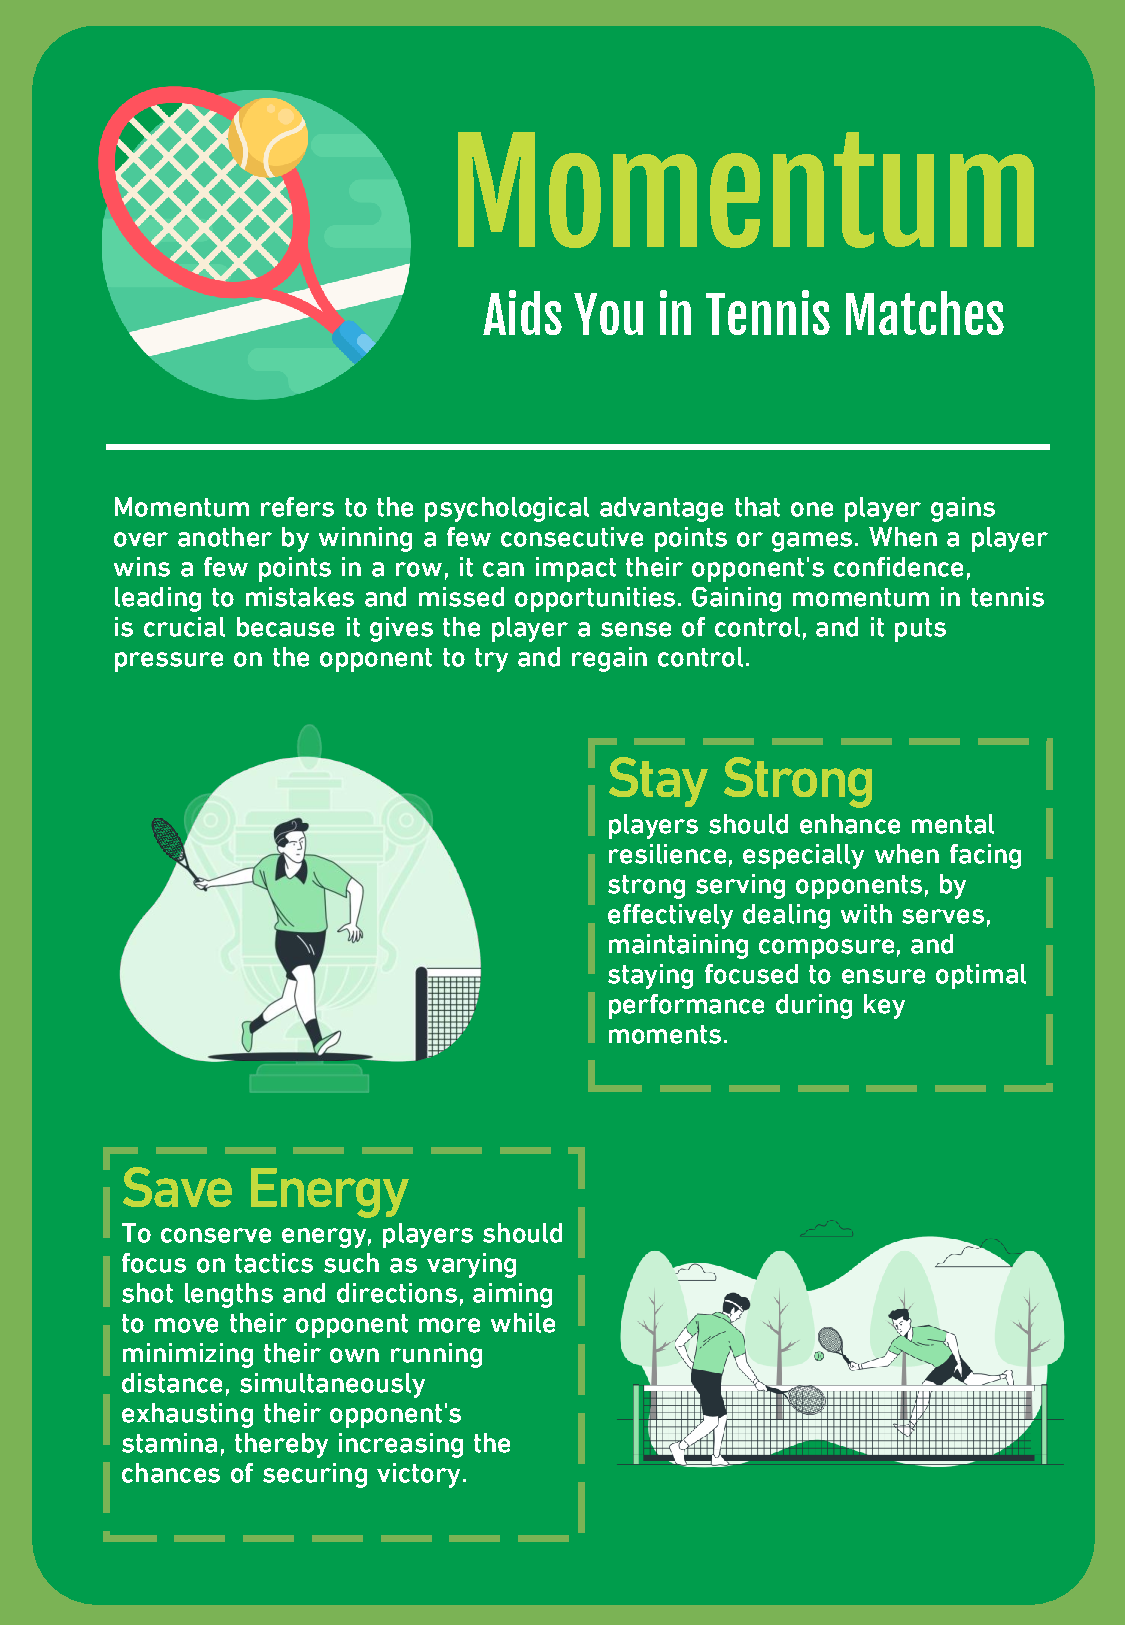
\includegraphics[width=\textwidth]{figures/memo.pdf} % 调整宽度为页面宽度    
\end{figure}
%%%%%%%%%%%%%%%%%%%%%%%%%%%%%%%%%%%%%%%%%%%%%%%%%%%%%%%

\newpage
\newpage
\printbibliography  % 打印引用文献列表
\bibliographystyle{unsrt}
\bibliographystyle{ref}

%%%%%%%%%%%%%%%%%%%%%%% 正文结束 %%%%%%%%%%%%%%%%%%%%%%%

\newpage
\newpage
\begin{appendices}  % 附录
\section{the code of Momentum Model and Performance Model}  % 一级标题

% Here are simulation programmes we used in our model as follow.\\
data processing
\textbf{Python source code:}
\lstinputlisting[language=Python]{./code/upload_data_cleanup_and_generate.py}


% \textbf{Python source code:}
% \lstinputlisting[language=C++]{./code/python.py}

\end{appendices}  % 附录结束
%%%%%%%%%%%%%%%%%%%%%%%%%%%%%%%%%%%%%%%%%%%%%%%%%%%%%%%
\end{document}  % 文档结束
%%%%%%%%%%%%%%%%%%%%%%%%%%%%%%%%%%%%%%%%%%%%%%%%%%%%%%%